\PassOptionsToPackage{utf8}{inputenc}
\documentclass{bioinfo}

\usepackage[draft]{hyperref}
\hypersetup{colorlinks=true,urlcolor=black,linkcolor=black,citecolor=black}
\usepackage{makecell}
\usepackage{comment}

\usepackage{floatrow}

% singlelinecheck=false puts subcaptions on the left
\usepackage[singlelinecheck=false]{subcaption}

\usepackage{algorithm2e}
\usepackage[usenames,dvipsnames]{xcolor}

\usepackage{orcidlink}

% we squeeze our figures even more together
\captionsetup{belowskip=-2pt}

\SetAlgoLined
\SetKwProg{MyStruct}{Struct}{ contains}{end}

\newcommand{\vocab}{\textbf}
\newcommand{\red}[1]{{\textcolor{Red}{#1}}}
\newcommand{\FIXME}[1]{\red{[FIXME: #1]}}
\newcommand{\REVIEWED}[1]{{\textcolor{Red}{#1}}}

\def\labelitemi{--}

\copyrightyear{2022} \pubyear{XXXX}

\access{Advance Access Publication Date: Day Month Year}
\appnotes{Genome Analysis}

\begin{document}
\firstpage{1}

\subtitle{Genome Analysis}

\title[ODGI: understanding pangenome graphs]{ODGI: understanding pangenome graphs}
\author[Guarracino, Heumos \textit{et~al}.]{
Andrea~Guarracino\orcidlink{0000-0001-9744-131X}\,$^{\text{\sfb 1} \dagger}$,
Simon~Heumos\orcidlink{0000-0003-3326-817X},$^{\text{\sfb 2} \dagger}$
Sven~Nahnsen\orcidlink{https://orcid.org/0000-0002-4375-0691}$^{\text{\sfb 2,3}}$,
Pjotr \\Prins\orcidlink{0000-0002-8021-9162}$^{\text{\sfb 4}}$,
and~Erik~Garrison\orcidlink{0000-0003-3821-631X}$^{\text{\sfb 4}*}$
}

\address{
$^{\text{\sf 1}}$Genomics Research Centre, Human Technopole, Milan, Italy \\
$^{\text{\sf 2}}$Quantitative Biology Center (QBiC), University of T\"ubingen, T\"ubingen, Germany, 72076 \\
$^{\text{\sf 3}}$Biomedical Data Science, Dept. of Computer Science, University of T\"ubingen, T\"ubingen, Germany, 72076 \\
$^{\text{\sf 4}}$University of Tennessee Health Science Center, Memphis, TN, USA
}

\corresp{$^\ast$To whom correspondence should be addressed. \\
$^\dagger$Contributed equally.}

\history{Received on XXXXX; revised on XXXXX; accepted on XXXXX}

\editor{Associate Editor: XXXXXXX}

% XXX key message of the paper is that we have collected a set of algorithms that enable easy use of pangenome graphs for investigating biology

\abstract{
\textbf{Motivation:}
Pangenome graphs provide a complete representation of the mutual alignment of collections of genomes.
These models offer the opportunity to study the entire genomic diversity of a population, including structurally complex regions.
Nevertheless, analyzing hundreds of gigabase-scale genomes using pangenome graphs is difficult as it is not well-supported by existing tools.
Hence, fast and versatile software is required to ask advanced questions to such data in an efficient way. \\
\textbf{Results:}
We wrote ODGI, a novel suite of tools that implements scalable algorithms and has an efficient in-memory representation of DNA \REVIEWED{pangenome graphs in the form of variation graphs}.
ODGI includes tools for detecting complex regions, extracting \textit{loci}, removing artifacts, exploratory analysis, manipulation, validation, and visualization.
Its fast parallel execution facilitates routine pangenomic tasks, as well as pipelines that can quickly answer complex biological questions of gigabase-scale pangenome graphs. \\
\textbf{Availability:}
ODGI is published as free software under the MIT open source license.
Source code can be downloaded from \url{https://github.com/pangenome/odgi} and documentation is available at \url{https://odgi.readthedocs.io}.
ODGI can be installed via Bioconda \url{https://bioconda.github.io/recipes/odgi/README.html} or GNU Guix \url{https://github.com/ekg/guix-genomics/blob/master/odgi.scm}. \\
\textbf{Contact:} \href{egarris5@uthsc.edu}{egarris5@uthsc.edu} \\
%\textbf{Supplementary information:} Supplementary data are available at \textit{Bioinformatics} online.
\\
\REVIEWED{\textbf{Keywords:} Navigating Variation Graphs. Pangenomic Liftover. Gigabase-Scale Pangenome Visualization. T2T Pangenome Graph Exploration.}
}

\maketitle

\section{Introduction}
A pangenome models the full set of genomic elements in a given species or clade~\REVIEWED{\citep{cpang2018,Eizenga_2020}}.
In contrast to reference-based approaches which relate \REVIEWED{samples} to a single genome, these data structures encode the mutual relationships between all the genomes represented.
\REVIEWED{[2,5] A class of methods to represent pangenomes involves the sequence graphs~\citep{Hein1989, Paten:2017}, where homologous regions between genomes are compressed into a single representative of all alleles present in the pangenome.
In node-labeled sequence graphs, nodes indicate \REVIEWED{[1,2] genomic sequences [1,2]}, with edges connecting the nodes that are concatenated in the sequences represented in the graph.
A bidirected sequence graph can \REVIEWED{[1,2] represent both strands of the genomic sequences [1,2]}.
On this model, variation graphs add the concept of paths representing linear \REVIEWED{[1,2] genomic [1,2]} sequences as traversals through the nodes of the graph~\citep{Garrison:2018}. \REVIEWED{[1,2] For example, a [1,2]} path can be a genome, haplotype, contig, or read. [2,5]}

\REVIEWED{Pangenome graphs can be constructed by multiple sequence alignment~\citep{Lee_2002,Grasso_2004} or by transitively reducing an alignment between sequences to an equivalent, labeled sequence graph~\citep{Kehr_2014,Garrison_2019_thesis}.
Current methods to build these graphs are still under active development~\citep{Li:2020,Armstrong:2020,pggb}, but they have largely settled on a common data model, represented in the Graphical Fragment Assembly (GFA) format~\citep{GFA}.
This standardization supports the development of a reference set of tools that operate on the pangenome graph model.}

Pangenome graphs let us encode any kind of variation, allowing the generation of comprehensive data systems that builds the basis for the analyses of genome evolution.
The Human Pangenome Reference Consortium (HPRC) and Telomere-to-Telomere (T2T) consortium~\citep{Miga:2020, Logsdon_2021, Nurk_2021} have recently demonstrated that high-quality \textit{de novo} assemblies can be routinely generated from third-generation long read sequencing data.
We anticipate that \textit{de novo} assemblies of similar quality will become common, leading to demand for methods to \REVIEWED{analyze} pangenomes.

Although \REVIEWED{pangenome graphs} are data structures of utility to researchers~\citep{cpang2018,Garrison:2018,Baaijens_2019,Hickey:2020,Sibbesen_2021}, the scientific community still lacks a toolset \REVIEWED{capable of operating on gigabase-scale pangenome graphs constructed from whole-genome assemblies}.
Such an effort began with the VG toolkit~\citep{Garrison:2018}\REVIEWED{, but its tools do not handle efficiently pangenome graphs presenting complex motifs that result from repetitive sequences like centromeres.}
Here we refocus it with the Optimized Dynamic Genome/Graph Implementation (ODGI) toolkit, a compatible, but independent pangenome graph interrogation and transformation system specifically implemented to handle the data scales encountered when working \REVIEWED{[1,10]with previously constructed pangenomes comprising hundreds of haplotype-resolved genomes.[1,10]}
ODGI offers a set of standard operations on the variation graph data model, generalizing ``genome arithmetic'' concepts like those found in BEDTools~\citep{Quinlan_2010} to work on pangenome graphs,
and providing a variety of operations, such as visualization, sorting, and liftover projections, all critical to understand and exploit pangenome graphs.

%Tools in ODGI operate on an efficient dynamic HandleGraph model \citep{Eizenga_2020_BX}.
%Algorithms written against this abstract API can be applied to the graph.% applies algorithms based on the HandleGraph API.
%This common API lets us reuse and and extend algorithms shared with the VG toolkit (VG) \citep{Garrison:2018}.
%We specifically develop new methods focused on problems encountered when building pangenome graphs at the scale of vertebrate populations.
%To ease interactive use, the majority of the ODGI's tools are implemented in an index-free manner, avoiding the need to create index structures at each step of complex graph processing pipelines.
%Thanks to ODGI's efficient path representation, its tools can work with variation graphs with highly complex regions.
%This eliminates one of the major bottlenecks when working with very large and deep variation graphs, and allows researchers to build and understand graphs of previously-inaccessible complexity and scale.

%\footnote{\url{https://humanpangenome.org/} (accessed Oct 2021)}
%\footnote{\url{https://sites.google.com/ucsc.edu/t2tworkinggroup/home} (accessed Oct 2021)}.

\section{Model}
A pangenome graph is a sequence model that encodes the mutual alignment of many genomes~\citep{Garrison_2019_thesis,Eizenga_2020}.
In the variation graph, $V = (N, E, P)$, nodes $N = n_1\ldots n_{|N|}$ contain \REVIEWED{[1,2] genomic sequences. [1,2]}
Each node $n_i$ has an identifier $i$ and an implicit reverse complement $\bar{n_i}$, and a node strand $s$ corresponds to one such orientations.
Edges $E = e_1\ldots e_{|E|}$ represent ordered pairs of node strands: $e_i = ( s_a, s_b )$.
Paths $P = p_1\ldots p_{|P|}$ describe walks over node strands: $p_i = s_1 \ldots s_{|p_i|}$.
When used as a pangenome graph, $V$ expresses sequences, haplotypes, contigs, and annotations as paths.
%The utility of the variation graph model lies in its lossless representation of genomes and their alignment.
By containing both the sequences and information about their relative variations, the variation graph provides a complete and powerful foundation for many bioinformatic applications.

%A more general approach is to build the graph from an alignment between sequences.
%We first transitively collapse characters in the input sequences that align together into single character in the output genome
%By projecting input sequences through this transformation, we obtain paths that losslessly encode the original sequences, but in the space of the graph \citep{Garrison_2019_thesis}.

\section{Implementation}
The ODGI toolkit builds on existing approaches to efficiently store and manipulate \REVIEWED{[2,5] pangenome graphs in the form of [2,5]} variation graphs~\citep{Garrison:2018}.
Similar to other efficient libraries presenting the \textsc{HandleGraph} model~\citep{Eizenga_2020_BX}, the implementation of ODGI's tools rests on three key properties which hold for most pangenome graphs:

\begin{enumerate}
\item They are relatively sparse, with low average node degree.
\item They can be sorted so that most edges go between nodes that are close together in the sort order.
\item Their embedded paths are locally similar to each other.
\end{enumerate}

These properties are used to build efficient dynamic variation graph data structures~\citep{Siren:2020,Eizenga_2020_BX}.
Sparsity (1) allows us to encode edges $E$ using adjacency lists rather than matrices or hash tables.
The local linear structure of the graph (2) lets us assign node identifiers that increase along the linear components of the graph, which supports a compact storage of edges and path steps as relativistic (usually small) differences rather than absolute (always large) integer identifiers.
Path similarity (3) allows us to write local compressors that reduce the storage cost of collections of path steps.
%\FIXME{without a figure we may lose the reader here a little} -- see algorithm 1

ODGI improves on prior efforts, based on issues that arose during our work with high-quality \textit{de novo} assemblies that cover almost all parts of the human genome~\citep{Logsdon_2021,Nurk_2021}.
In particular, we find that it is necessary to support graphs with regions of very high numbers of path traversals (high path depth).
Such motifs can occur in collapsed structures generated by ambiguous sequence homology relationships in repeats found in the centromeres and other segmental duplications.
If we cannot process such regions, there are only two options: 1) remove such regions, or 2) leave them unaligned.
However, neither of these solutions allows us  their biological features.
To seamlessly represent such difficult regions, we followed an approach implemented in the dynamic version of the Graph BWT (GBWT)~\citep{Siren:2020} and built a node-centric, dynamic, compressed model of the paths.
This design supports node-local modification and update of the graph, which lets us operate on paths in parallel.

We store the graph in a vector of node structures, each of which presents a node-local view of the graph sequence, topology, and path layout.
Expressed in terms of the variation graph $V$, ODGI's core $Node$ structure includes a decoder that maps the neighbors of each node to a dense range of integers.
For a given $Node_i$ and neighbor $Node_j$, the decoder itself does not store the $id$ of $Node_j$, but rather a compact representation of the relative difference between the node ids: $\delta = Node_i.id - Node_j.id$.
%The $\delta between two nodes is computed as their distance in the graph vector (i.e., the difference between the node offsets).
This keeps the size of the encoding small, per common pangenome graph property (2).
We define the edges and path steps traversing the node in terms of this alphabet of $\delta$'s.
The structures in Algorithm~\ref{alg:structs} describes our encoding.

\begin{algorithm}
\MyStruct{Node}{
    \textbf{id} $\in \mathbb{N}$ \tcp{an identifier}
    \textbf{lock} \tcp{atomic locking primitive}
    \textbf{sequence} $= [$A$|$T$|$G$|$C$|$N$]*$ \\
    \tcp{bit-packed vector of edges}
    \textbf{edges} $= (x_i,x_j)* : (i, j) \in [1\ldots \Sigma]^2$ \\
    \tcp{bit-packed vector of id deltas}
    \textbf{decoding} $x_1 \ldots x_{\Sigma} \in \mathbb{N}^\Sigma$ \\
    \tcp{bit-packed vector of path steps}
    \textbf{path\_steps} $[Step_1 \ldots Step_n]*$
}
\MyStruct{Step}{
    \textbf{path\_id} $\in \mathbb{N}$ \tcp{the path's global id}
    \textbf{is\_rev} $\in ( 0, 1 )$ \tcp{the step orientation}
    \textbf{is\_start} $\in ( 0, 1 )$ \tcp{if first step in path}
    \textbf{is\_end} $\in ( 0, 1 )$ \tcp{if last step in path}
    \textbf{prev\_$\delta$} $\in [1\ldots \Sigma]$ \tcp{$\delta$-encoded previous node}
    \textbf{prev\_rank} $\in \mathbb{N}$ \tcp{step rank on previous node}
    \textbf{next\_$\delta$} $\in [1\ldots \Sigma]$ \tcp{$\delta$-encoded previous node}
    \textbf{next\_rank} $\in \mathbb{N}$ \tcp{step rank on next node}
}
\caption{ODGI's relativistically-packed $Node$ structure and the $Step$ structure used to represent the paths as doubly-linked lists.}
\label{alg:structs}
\end{algorithm}

Each structure contains the sequence of the node ($Node_i.sequence$), its edges in both directions ($Node_i.edges$), and a vector of path steps that describes the previous and next steps in paths that walk across the node ($Node_i.path\_steps$).
For efficiency, $Node_i.sequence$ is stored as a plain string, while the $edges$ and $path\_steps$ are stored using a dynamic succinct integer vector that requires $O(2nw)$ bits for the edges and $O(5nw)$ bits for the path steps, where $n$ is the number of steps on the node and $w$ is $\approx log_2(n)$ \citep{prezza2017framework}.

To allow edit operations in parallel, each node structure includes a byte-width mutex $lock$.
All changes on the graph can involve at most two $Node$ structs at a time (both edge and path step representations are doubly-linked).
To avoid deadlocks, we acquire the node locks in ascending $Node.id$ order and release them in descending order.
In addition to node-local features of the graph, we must maintain some global information.
Specifically, we record the start and end of paths, as well as a name to path id mapping in lock-free hash tables.
The use of lock-free hash tables lets us avoid a global lock when looking up path or graph metadata, which would quickly become a bottleneck during parallel operations on the graph.
By avoiding global locks, we implement many of the operations in ODGI using maximum parallelism available.
This approach is key to enable our methods to scale to the largest pangenome graphs that we can currently build (with hundreds of vertebrate genomes).

%\subsection{Core functionality}
%In the variation graph model, paths have to respect the graph’s topology: this can be verified with odgi validate, to ensure no errors in the input or edited graphs.
%In variation graphs the coordinates are provided by the embedded path sequences.
%Indeed, the node IDs are not meant to be stable. odgi position finds, translates, and liftovers graph and path positions between different graphs by exploiting their shared path sequences (Figure 1.B).

\begin{comment}
key message of the paper is that we have collected a set of algorithms that enable easy use of pangenome graphs for investigating biology
-> build model solves problem of working with big graphs in memory
-> view (convert to GFA) & paths solve problem of exporting basic features of the graph (e.g. paths)
-> stats (understand basic size / structure) & bin & degree & depth solves problem of understanding the overall structure and size of the graph
-> sort (groom) & layout solves problem of finding latent structure in the pangenome
-> viz & draw provides a human-viewable readout of the graph
-> chop & unchop & squeeze & break & prune & explode lets us break apart or combine the graph nodes and topology
-> position & tips & untangle (jaccard based coordinate conversion) provides a way to map coordinates between any genomes in the graph (e.g. liftover!)
-> extract lets us pull out specific regions of the graph based on path ranges, nodes and positions
\end{comment}

\begin{figure*}[ht!]
  %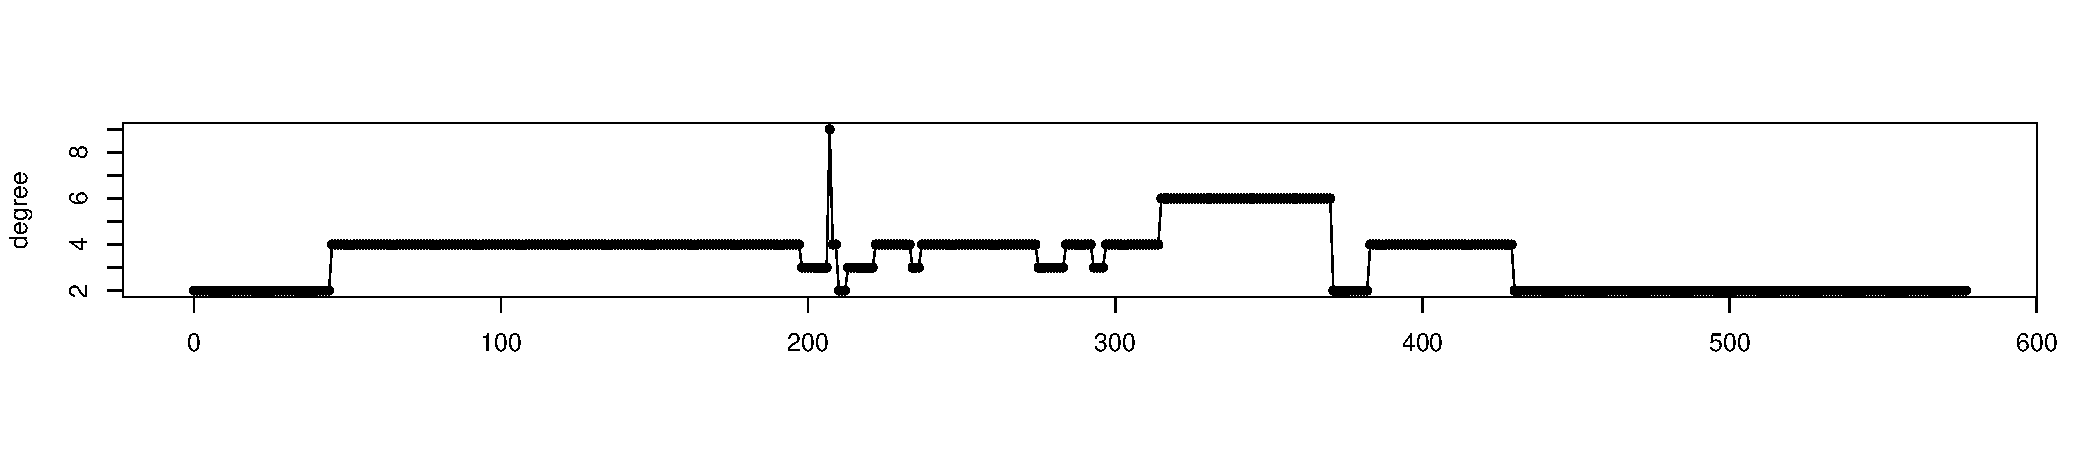
\includegraphics[width=\linewidth,trim=+.225cm 0 +.425cm +2cm]{fig/metrics/chr4_HTT_chm13_degree_w1_bed.pdf}  
  \includegraphics[width=\linewidth]{fig/odgi_tools.pdf}
  \caption{Methods provided by ODGI (in black) and their supported input and output data formats (in brown).}
  \label{fig:operations}
\end{figure*}


\section{Results}

ODGI provides a set of interrogative and manipulative operations on pangenome graphs.
We have established these tools to support our exploration of graphs built from hundreds of large eukaryotic genomes.
ODGI's tools are practical and able to work with high levels of graph complexity, even with regions where paths present very high depth nodes (10$^5$ to 10$^6$-fold depth).

ODGI covers common operations that we have found to be essential when working with complex pangenome graphs:

\begin{itemize}
\item \textit{odgi build} constructs the ODGI data model from GFA file (\S\ref{sec:build}).
\item \textit{odgi view} converts the ODGI data model into GFA file (\S\ref{sec:build}).
\item \textit{odgi viz} provides a linear visualization of the graph (\S\ref{sec:viz}).
\item \textit{odgi draw} renders a 2D image of the graph (\S\ref{sec:viz}).
\item \textit{odgi extract} excerpts subsets of the graph based on path ranges (\S\ref{sec:extract}).
\item \textit{odgi explode} breaks the graph into connected components (\S\ref{sec:extract}).
\item \textit{odgi squeeze} unifies disjoint graphs (\S\ref{sec:extract}).
\item \textit{odgi chop} breaks long nodes into shorter ones (\S\ref{sec:edit}).
\item \textit{odgi unchop} combines unitig nodes (\S\ref{sec:edit}).
\item \textit{odgi break} removes cycles in the graph (\S\ref{sec:edit}).
\item \textit{odgi prune} removes complex regions (\S\ref{sec:edit}).
\item \textit{odgi groom} resolves spurious inverting links (\S\ref{sec:edit}).
\item \textit{odgi position} lifts coordinates between path and graph positions (\S\ref{sec:untangle}).%
%\item \textit{odgi server} provides a HTTP server to lift coordinates (\S\ref{sec:untangle}).
\item \textit{odgi untangle} deconvolutes paths relative to a reference (\S\ref{sec:untangle}).
\item \textit{odgi tips} finds path end points relative to a reference (\S\ref{sec:untangle}).
\item \textit{odgi sort} orders the graph nodes (\S\ref{sec:sort}).
\item \textit{odgi layout} establishes a 2D layout (\S\ref{sec:sort}).
\item \textit{odgi matrix} derives the pangenome matrix (\S\ref{sec:metrics}).
\item \textit{odgi paths} lists and extracts paths in FASTA (\S\ref{sec:metrics}).
\item \textit{odgi flatten} converts the graph to FASTA and BED (\S\ref{sec:metrics}).
\item \textit{odgi stats} provides numerical properties of the graph (\S\ref{sec:metrics}).
\item \textit{odgi bin} generates a summarized view of the graph (\S\ref{sec:metrics}).
\item \textit{odgi depth} describes node depth over graph and path positions (\S\ref{sec:metrics}).
\item \textit{odgi degree} describes node degree over graph and path positions (\S\ref{sec:metrics}).
\end{itemize}

Each tool focuses on a small set of related operations.
Most read or write the native ODGI format (`og' extension) (Figure~\ref{fig:operations}) and work with standard text based data formats common to bioinformatics.
This supports the implementation of flexible and composable graph processing pipelines based on graphs (GFA/ODGI) and standard bioinformatic data types representing positions, genomic ranges (BED), and pairwise mappings (PAF).
%While the pangenome graph is a first-class entity in ODGI,
% develop a universal, stable, coordinate system, rendering these data types relative to reference and query sequences embedded in the graph.
%To develop a stable and compatible coordinate system, 
We use variation graph paths to provide a universal coordinate system, representing annotations and pairwise sequence relationships using the paths as reference and query sequences.
%This avoids the complexity of establishing a stable coordinate system over the topology of the graph, which may change when it is modified or subset.
%Although they present new complexities, we find that pangenome graphs are compatible with current standard ways of working with bioinformatics data.
Thus, ODGI provides a set of interfaces that let us approach these graphs from the perspective of standard reference- and sequence-based data models.
Indeed, by considering all paths in the graph as potential reference or query sequence, we make graphs invisible to downstream tools that operate on collections of sequences or rely on a reference sequence (\textit{e.g.} SAMtools~\citep{Li2009}), enabling interoperability.
This approach benefits from the information in the graph without strongly embedding our methods in this difficult new research context.

%We begin with a set of HandleGraph-based algorithms first establish in the VG toolkit \citep{Garrison:2018}.
%These include algorithms for graph traversal, partition-finding, $k$-mer and character enumeration, sorting, and pruning.
%Unlike VG, we provide no methods to construct graphs, map reads to the graph, or derive variants.

%Most of the tools are designed to be applied together, piping the output of one tool into the next, thereby preventing the creation of intermediate files, and reducing the number of IO operations.


\subsection{Building the \textsc{ODGI} model}
\label{sec:build}
ODGI maintains its own efficient binary format for storing graphs on disk.
We begin by transforming the storage model of the standard GFAv1~\citep{GFA} format (in which nodes, edges, and paths are described independently) into the ODGI node-centric encoding with \textit{odgi build}.
This construction step can be a significant bottleneck, in particular as the size of the path set of the graph increases. \REVIEWED{[1,5]The process itself is lossless. A graph in ODGI format represents everything that is in the input GFAv1 graph, without any loss of information.[1,5]} \REVIEWED{[2,1]ODGI does not support GFAv2 nor rGFA. The less popular GFAv2 format was specifically designed for assembly graphs. rGFA requires a genomic sequence to be the reference sequence, but in GFAv1 we don't have that limitation which is fundamental to implement reference-free approaches.[2,1]}

The ODGI data structure (Algorithm~\ref{alg:structs}) allows algorithms that build and modify the graph to operate in parallel, without any global locks.
In \textit{odgi build}, we initially construct the node vector in a serial operation that scans across the input GFA file.
Then, we serially add edges in the $Node.edges$ vectors of pairs of nodes.
Finally, we create paths in serial, and extend them in parallel by obtaining the mutex $Node.lock$ for pairs of nodes and by adding the path step in their $Node.path\_steps$ vectors.
This parallelism speeds ODGI model construction by many-fold when testing against graphs made from assemblies produced by the HPRC (Figure~\ref{fig:build}).

To support interchange with other pangenome tools or text-based processing, \textit{odgi view} converts a graph in ODGI binary format to GFAv1.
%ODGI uses the ``S'' and ``L'' records to describe the graph topology, and ``P'' records to describe paths.

\begin{figure}[h!]
	\centering
	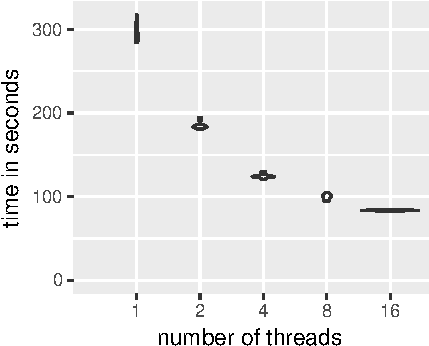
\includegraphics[width=\linewidth]{fig/build/mean_build_time.pdf}
	\caption{Performance evaluation of \textit{odgi build} when translating a 90 haplotypes human chromosome 6 graph into ODGI's native format. The error margins are the standard deviations computed from 10 runs for each of the different threading configurations.}
	\label{fig:build}
\end{figure}


\subsection{Visualizing pangenome graphs}
\label{sec:viz}

% interesting that we don't go base-level at all... we use vg for that, or STM

Pangenome graph visualization is one of the first steps to gain insight into the mutual relationship between the sequences in the graph and their variation.
We pursue a novel approach to visualization with \textit{odgi viz} and \textit{odgi draw}, two tools which provide scalable ways of generating \REVIEWED{static} pictures of the high-level structure of large pangenome graphs.

\textit{odgi viz} supports a binned, linearized rendering in 1 dimension (1D) (that is, all graph nodes lie on the same axis).
This visualization is computed in linear-time and offers a human-interpretable format suitable for understanding the topology and genome relationships in the pangenome graph (Fig.~\ref{fig:odgi_viz}).
Graph nodes are arranged on a single axis, from left to right, with the colored bar indicating the paths and the nodes they cross.
White spaces indicate where paths do not traverse the nodes.
The meaning of the colors depends on how \textit{odgi viz} is executed.
By default, path colors are derived from the path names (Fig.~\ref{fig:odgi_viz}\textbf{b}).
Path names are displayed on the left of the paths.
The black lines on the bottom indicate the edges connecting the nodes and, therefore, represent the graph topology.

Nevertheless, complex, nonlinear graph structures are difficult to display and interpret in a low number of dimensions.
To overcome such a limitation, \textit{odgi viz} supports multiple visualization modalities (Fig.~\ref{fig:odgi_viz}\textbf{c-e}), making it easy to grasp the properties and shape of the graph.
Graph node order can affect downstream analyses on pangenome graphs.
With \textit{odgi viz} we can color the paths by path position (Fig.~\ref{fig:odgi_viz}\textbf{c}), with light grey indicating where paths begin and dark grey where they end.
This visualization is suitable for understanding graph node order, as smooth color gradients indicate that the graph order respects the linear paths' coordinate systems.
Pangenome graphs represent both strands \REVIEWED{[1,2] of the genomic sequences [1,2]}.
\textit{odgi viz} supports also coloring the paths by orientation, with paths colored where their sequence is reverse-complemented (red) or in direct orientation (black) with respect to the sequences of the graph nodes (Fig.~\ref{fig:odgi_viz}\textbf{d}).
Eukaryotic genomes experience gains and losses of genetic material, resulting in copy number variation (CNV) across the population.
With \textit{odgi viz}, we can use multiple color palettes to color the paths by path depth, highlighting the different copy number statuses in the \REVIEWED{[1,2] genomic sequences [1,2]} represented in the pangenome graph (Fig.~\ref{fig:odgi_viz}\textbf{e}).

\textit{odgi draw} extends the visualization in 2 dimensions (2D)  (Fig.~\ref{fig:odgi_viz}\textbf{a}) by rendering the layout built by \textit{odgi layout} (\S\ref{sec:sort}).
A 2D rendering is more costly to compute, but we similarly provide an implementation that scales linearly with pangenome sequence size, allowing us to apply it to large pangenome graphs.


\subsection{Extracting or joining regions of interest}
\label{sec:extract}

Pangenome graphs built from hundreds of haplotype-resolved \textit{de novo} genome assemblies are very large, but it is often necessary to work with only a small portion of the genomes represented,
such as a specific \textit{locus} (Fig.~\ref{fig:odgi_viz}\textbf{a}) or a smaller region (Fig.~\ref{fig:odgi_viz}\textbf{b-g}), or even a single gene (Fig.~\ref{fig:metrics}).
This simplifies the downstream analyses and reduces the resources to work only with the extracted graphs.
%Subsetting operations allow us to zoom in on particular genes or regions of interest for more precise examination.
Graph portions can be extracted by using the paths in the graph as coordinate systems to guide the process. For such operation, \textit{odgi extract} allows users to extract specific regions of the graph as defined by query criteria.
Regions of interest can be specified by graph nodes or path range(s), also in BED format. Furthermore, it is possible to indicate a list of paths to be preserved completely in the extracted graph.

In \textit{odgi extract}, we begin by collecting all graph nodes that fall within the ranges to extract (and the paths to preserve, if requested).
Users can specify the number of steps or nucleotides to expand the selection and include neighboring nodes.
Then, edges connecting all selected nodes are added in the subgraph under construction.
Finally, the portions of the paths (\textit{i.e.}, the subpaths) walking through the selected nodes are extracted and added to the new subgraph.
Subpaths are searched in parallel, created serially, and extended in parallel again thanks to the parallelism enabled by the ODGI data structure (see \S\ref{sec:build}), making \textit{odgi extract} a scalable solution to extract also complex subregions presenting nodes with very high path depth.

% If needed, we can have a figure showing extraction process---either schematic or ``real''.

Pangenome graphs can embed multiple chromosomes as separated connected components (inter-chromosomal structural variants would join the components into bigger ones).
\textit{odgi explode} separates the connected components in different ODGI format files, while \textit{odgi squeeze} allows merging multiple graphs into the same ODGI format file, preventing node ID collisions.


\subsection{Editing the graph structure}
\label{sec:edit}

Pangenome graphs can be used in a variety of applications, ranging from read mapping to variant identification and genotyping~\citep{Eizenga_2020}.
However, graphs presenting complex topology can increase the computational overhead of many downstream analyses.
ODGI offers multiple commonly-needed basic operations on the topology of the graph and its nodes.

For simplifying the graph structure, users can use \textit{odgi prune} to take away complex parts as defined by query criteria,
while with \textit{odgi break} they can remove cycles in the graph, reducing the complexity of the graph topology.
Furthermore, \textit{odgi groom} allows removing spurious inverting links by exploring the graph from the orientation supported by most paths.

To enable efficient sequence alignment against the graph, long nodes can be divided into shorter nodes at a maximum requested size using \textit{odgi chop}.
Partial order alignment, which consists of aligning sequences against a directed acyclic graph (DAG), is frequently used in pangenome building pipelines~\citep{pggb}, but the current implementations return DAGs with 1-bp long nodes.
\textit{odgi unchop} allows joining nodes that can be merged without changing the graph topology, nor the embedded sequences, obtaining an equivalent, but more compact, representation of the graph.


\subsection{Untangling and navigating the pangenome}
\label{sec:untangle}

%We find that, to understanding relationships between sequences and positions in pangenome graphs, we must use context mapping to ``untangle'' complex regions found in VNTRs, segmental duplications, and centromeric repeats.
%This approach lets use pangenome graphs as a foundation for universal liftover between any two sets of sequences in the graph.

The key data in a pangenome graph is a representation of the alignment (or homology) relationships between the sequences represented.
Navigating and understanding the graph requires coordinate systems that we can use to link other data into the graph model, and thus to the \REVIEWED{[1,2] genomic sequences [1,2]} in the pangenome.
ODGI's tools use the embedded sequences to provide a universal coordinate space that is graph-independent, thereby remaining stable across different graphs built with the same genomes.
%Our for positional conversion (\textit{odgi position}), annotation liftover (\textit{odgi untangle}), breakpoint identification (\textit{odgi tips}), subgraph extraction (\textit{odgi extract}), visualization (\textit{odgi viz}), path depth (\textit{odgi depth}), and graph complexity measurement (\textit{odgi degree}) can all operate on coordinates of paths in the graph.

A universal coordinate system allows us to support several kinds of ``lift-over'' of coordinates between different genomes in the same or different graphs.
%For basic liftover operations, \textit{odgi server} provides a basic HTTP server that can translate very efficiently a path position to a pangenomic position within the same graph.
\textit{odgi position} translates graph and path positions between or within graphs, emitting the liftovers in BED format.
Coordinates can be specified in BED format, but users can even specify a GFF/GTF file to project the annotations into the pangenome graph (Fig.~\ref{fig:odgi_viz}\textbf{f-g}). 

For a precise translation process when conversing a query position to a reference position in a repeat region, we apply the \textit{path jaccard} context mapping concept.
It could be that the found reference node is visited several times by the reference.
To ensure a precise translation, we select the reference position whose context (the multiset of $Node.id$s reached within a distance of e.g. 10kbp) has the best jaccard metric when compared to the query context.
%the best jaccard for the query step and each reference candidate step is calculated by looking at a context range (e.g. 10kbp) around the locus.

% untangle (this follows on the jaccard graph mapping concepts in the previous section}
%We can use coordinates in any genome to refer to it, but this requires a few basic operations ...
%Obtaining unambiguous mappings between different genomes requires the use of a new kind of graph based mapping (path graph jaccard).

Pangenome graphs \REVIEWED{can} model alignments of many genomes.
With \textit{odgi untangle}, users can extract pairwise alignment information between a given set of ``query'' sequences and a given set of ``target'' sequences (used as references).
While pangenome graphs may contain looping structures that imply many-to-many alignments between the pangenome sequences, these untangled alignments map each segment of the queries to a single segment in the set of targets.
%This lets us decompose both homology and paralogy relationships by also untangling looping motifs in the graph, and obtaining linearized pairs of regions in BEDPE or PAF format.
Being able to work with any sets of reference sequences lets us convert the graph to lift-over maps compatible with standard software for projecting annotations and alignments from one genome to another.
As an example, by untangling the graph we can study the variation that lies in regions collapsed due to ambiguous alignments over sequence repeats (as shown in Fig.~\ref{fig:odgi_viz}\textbf{f}).
Indeed, to obtain a more precise overview of the \textit{locus} in Fig.~\ref{fig:odgi_viz}\textbf{b-e},
we can apply \textit{odgi untangle} to segment paths into linear segments by breaking these segments where the paths loop back on themselves.
We first discover segment boundaries using standard approaches for detecting repeats in sequence graphs \citep{Pevzner_2004}.
We finally ``untangle'' by finding the target segment that best match each query segment using the \textit{path jaccard} context mapping model.
%The \textit{path jaccard} concept ensures that the breaking is nucleotide-precise.
In this way, we obtain information on the position and copy number status of the sequences in the collapsed \textit{locus} (Fig.~\ref{fig:odgi_viz}\textbf{h}).
Moreover, to obtain base-level precise information on the relationships between the repeated sequences, we can align them by using the pairs of regions that came from the untangling to guide the alignment~\citep{wfmash}.

%Having built a pangenome graph from assembly contigs, we can ask questions like: Where do our contigs' ends match the reference(s)? An answer to this question can highlight regions that are tricky to assemble (Fig. ~\ref{fig:tips}). 
\textit{odgi tips} can identify the break point positions of the contigs relative to the reference(s) in the graph by walking from the ends of each contig until a reference node is found. 
It could be that the reference visits the node several times. Therefore, for each contig range (a tip) \textit{odgi tips} takes a look at each possible reference window and finds the most similar one using the \textit{path jaccard} concept. 
The output is a BED file with the best reference hit and position for each of the contigs' ends. 

\subsection{Sorting the pangenome graph}
\label{sec:sort}

Pangenome graphs can hide their underlying latent structures, introducing difficulties in the analysis and interpretation. % (Fig.~\ref{fig:sorting}\textbf{a}).
Among the causes of this is the correct ordering of the graph nodes in a convenient number of dimensions.
ODGI provides a variety of sorting algorithms to find the best graph node order in 1 or 2 dimensions, allowing us
to understand the sparse structures typically found in pangenome graphs and the genetic variation they represent.

To find the best order of graph nodes in 1D, \textit{odgi sort} provides multiple sorting algorithms which can be combined into a sorting pipeline to take advantage of the strength of each.
Most notably, nodes can be sorted topologically, randomly, by breaking cycles in the graph (\S\ref{sec:edit}), by grooming (\S\ref{sec:edit}), and/or by using a novel path-guided (PG) stochastic gradient descent (SGD) algorithm: PG-SGD.
This exploits path information to order the graph nodes.
%For understanding the large-scale organization of the graph, we benefit from an even simpler coordinate system.
PG-SGD learns a 1D or 2D organization of the graph nodes that matches distances in graph paths.
To scale to large graphs, we learn this projection in parallel via a HOGWILD! approach~\citep{niu2011hogwild}.
Our approach can be seen as an adaptation of SGD-based drawing to pangenome graphs~\citep{zheng2018graph}.
In parallel, each HOGWILD! thread updates node relative positions to best-match their nucleotide distance in the paths running through the graph.
Following standard SGD approaches, a learning rate is reduced as the algorithm progresses, and execution continues until the adjustments to the model fall below a target threshold $\epsilon$.
ODGI can project vector (in 1D) and matrix (2D) representations of the graph relative to these learned coordinate spaces.
Based on this projection, we can trivially sort graph nodes in 1D.
Moreover, we support the same concept in 2D in \textit{odgi layout} by providing a 2D implementation of the PG-SGD algorithm.
%As the PG-SGD sorts graph nodes with respect to the paths which walk through them, we can also detect regions whose layout is distorted, which may represent structural variation or assembly error.


\begin{figure}[ht!]
    \begin{subfigure}{\linewidth}
        \caption{}
        \centering
        % include first image
        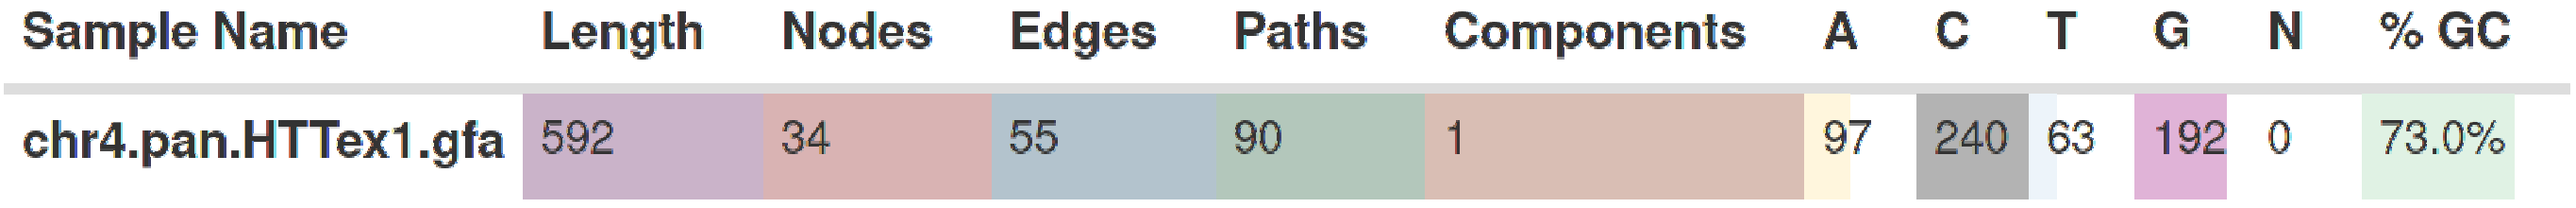
\includegraphics[width=1.0\linewidth, trim=-2.25cm 1.0cm 0cm 3.75cm]{fig/metrics/chr4_pan_HTTex1_gfa_multiqc_odgi_stats_svg}
        \label{fig:metrics-multiqc}
        	\vspace{-2em}
    \end{subfigure}
    \begin{subfigure}{1\linewidth}
        \caption{}
        \centering
        % include fourth image
        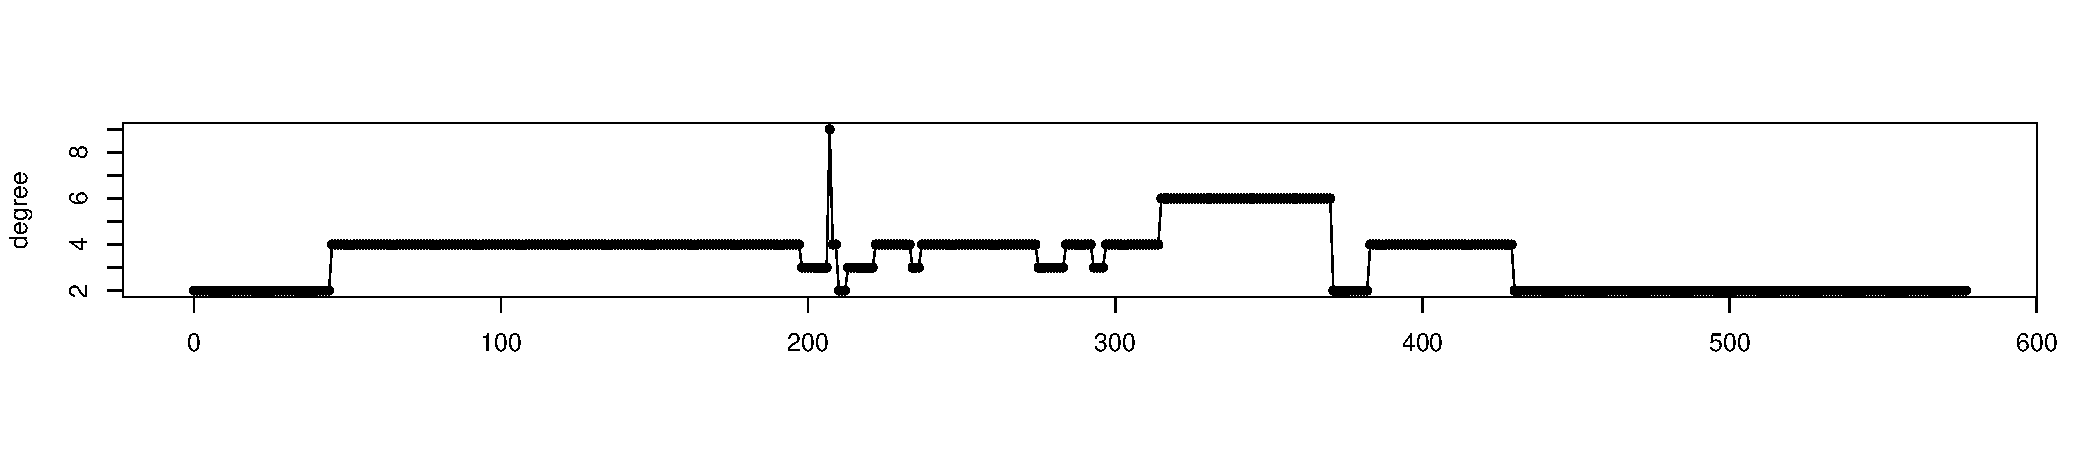
\includegraphics[width=\linewidth,trim=-.225cm 4cm +.425cm +3cm]{fig/metrics/chr4_HTT_chm13_degree_w1_bed}
        \label{fig:metrics-degree}
    \end{subfigure}
    \begin{subfigure}{\linewidth}
        \caption{}
        \centering
        % include second image
        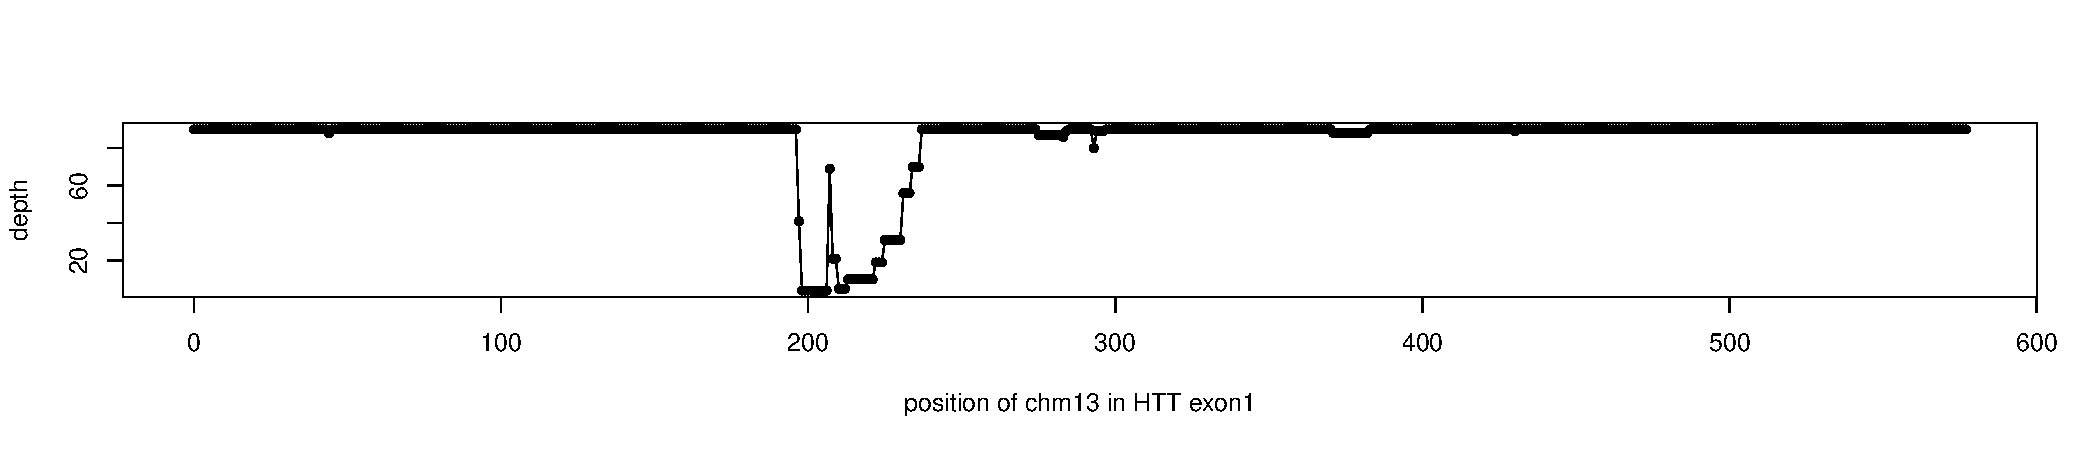
\includegraphics[width=\linewidth,trim=-.225cm 3.3cm +0.425cm +3cm]{fig/metrics/chr4_HTT_chm13_depth_w1_bed}
        \label{fig:metrics-depth}
    \end{subfigure}
    \begin{subfigure}{\linewidth}
        \caption{}
        \centering
        % include second image
        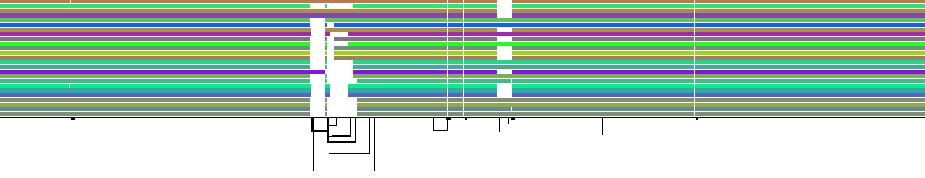
\includegraphics[width=1.0\linewidth, trim=-1.75cm 2.2cm -0.75cm 0.5cm]{fig/metrics/chr4_pan_fa_a2fb268_4030258_6a1ecc2_smooth_gfa_og_HTTex1_og_O_og_tiny_og_png_svg.pdf}
        \label{fig:metrics-viz}
    \end{subfigure}
    \begin{subfigure}{\linewidth}
        \caption{}
        \centering
        % include second image
        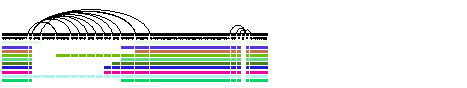
\includegraphics[width=1.0\linewidth, trim=-0.4cm 0.4cm 3.15cm 0cm]{fig/metrics/chr4_pan_HTTex1_STR_xg_svg}
        \label{fig:metrics-str}
        \vspace{-0.5em}
    \end{subfigure}
%	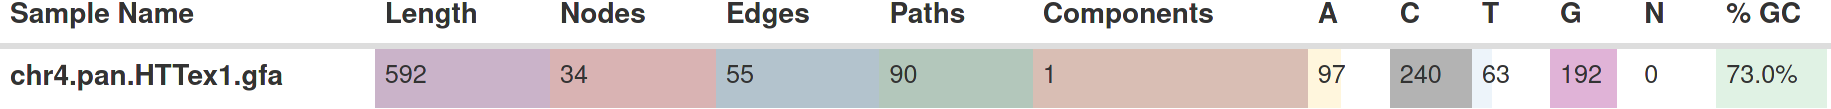
\includegraphics[width=\linewidth]{fig/metrics/chr4.pan.HTTex1.gfa.multiqc_odgi_stats.png}
	\caption{Features of a 90-haplotype human pangenome graph of the exon 1 huntingtin gene (\textit{HTTexon1}): \textbf{(a)} Excerpt of vital statistics of the \textit{HTTexon1} graph displayed by MultiQC's ODGI module. The very high GC content of 73.0\% compared to a human genomic mean GC content of 40.9\% \citep{Piovesan2019} is in accordance with the literature \citep{Neueder2017}. \textbf{(b)} Per nucleotide node degree distribution of CHM13 in the \textit{HTTexon1} graph. Around position 200 there is a huge variation in node degree. \textbf{(c)} Per nucleotide node depth distribution of CHM13 in the \textit{HTTexon1} graph. The alternating depth around position 200 indicates polymorphic variation complementing the above node degree analysis. \textbf{(d)} \textit{odgi viz} visualization of the 23 largest gene alleles, CHM13, and GRCH38 of the \textit{HTTexon1} graph. \textbf{(e)} \textit{vg viz} nucleotide-level visualization of 10 gene alleles, CHM13, GRCH38 of the \textit{HTTexon1} graph focusing on the CAG variable repeat region. Figures \textbf{(b)-(e)} highlight the variant region around position 200 of CHM13 showing the variable number of glutamine residues of the different individuals as reported by \citep{Nance1999}.}
	\label{fig:metrics}
\end{figure}


\subsection{Obtaining metrics of the pangenome graph}
\label{sec:metrics}

Graphs statistics provide alternative ways to gain insight into pangenomes complexity revealing the overall structure, size, and features of a graph and its sequences.

Pangenome graph topology can be derived by applying \textit{odgi matrix}, obtaining information on graph nodes connections in textual sparse matrix format.
To investigate on the \REVIEWED{[1,2] genomic sequences [1,2]} encoded in the graph, \textit{odgi paths} allows users to calculate pairwise overlap statistics of groupings of paths and emit all path sequences in FASTA format, and it also allows the generation of a ``pangenome matrix'' that reports the copy number (presence/absence) of each path over each node.
\textit{odgi flatten} generates a linearization of the graph by emitting the pangenome sequence (the concatenation of all node sequences) in FASTA format, and the projection of all paths on the linearized sequence in BED format.

Applying \textit{odgi stats}, users can retrieve metrics describing the graph properties, such as the number of nodes, edges, paths, and graph length.
It outputs pangenome statistics in tab-separated values (TSV) or YAML textual file formats.
MultiQC's~\citep{Ewels_2016} ODGI module %\footnote{\url{https://multiqc.info/docs/\#odgi} (accessed Oct 2021)}
provides an interactive way to comparatively explore such statistics of an arbitrary number of graphs.

ODGI also offers more advanced tools for the interrogation of the graphs.
To study very large pangenomes, users can use \textit{odgi bin} to summarize the path information into bins of a specified size, generating a summarized view of gigabase scale graphs in TSV or JSON file formats.
%This concept found its way into the pangenome graph ontology \cite{Yokoyama2020}. %maybe we want to save this up for the discussion

Genomes presenting sequences with highly identical repeats result in pangenome graphs with complex motifs that can be detected by \textit{odgi depth} and \textit{odgi degree}, which return the node depth and node degree, respectively, as defined by query criteria.
Both tools emit the output in BED format, allowing users to assess the complexity of the graph and detect intricate regions.
Indeed, high depth/degree nodes can be the mirror of genetic variation (Fig.~\ref{fig:metrics}), but also misassemblies or problems in the pangenome building, making the tools further useful for graph validation.
%In Fig.~\ref{fig:metrics}, the characteristics of a 90 haplotypes human pangenome graph of the exon 1 huntingtin gene~\citep{Sathasivam2013,Neueder2017} (\textit{HTTexon1}) are shown.


\begin{figure*}[!htb]
    \centering
    \begin{tabular}[t]{c}%{|c|c|}
        %\hline
        \begin{subfigure}[t]{1.0\textwidth}
            \centering
            \caption{\label{fig:odgi_layout}}
            
\includegraphics[width=\linewidth, trim=0cm 18cm -20cm 0.5cm]{fig/extract_viz_draw_position_untangle/chr6_pan_fa_a2fb268_4030258_6a1ecc2_smooth_mhc_H1000w120}
        \end{subfigure} \\
        \begin{tabular}{c}% if you add [t], then sub images are pushed down
            %\smallskip
            \begin{subfigure}[t]{0.5\textwidth}
                \centering
                \caption{}
                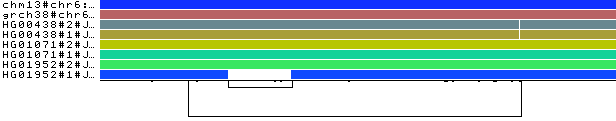
\includegraphics[width=\linewidth, trim=0 1.9cm 0cm 0cm]{fig/extract_viz_draw_position_untangle/chr6_pan_fa_a2fb268_4030258_6a1ecc2_smooth_C4_sorted}
            \end{subfigure} \\
            \begin{subfigure}[t]{0.5\textwidth}
                \centering
                \caption{}
                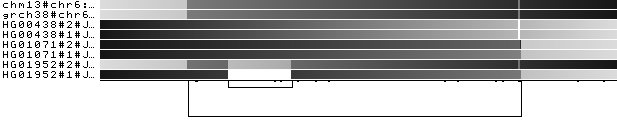
\includegraphics[width=\linewidth, trim=0 +1.9cm 0cm 0cm]{fig/extract_viz_draw_position_untangle/chr6_pan_fa_a2fb268_4030258_6a1ecc2_smooth_C4_sorted_du}
            \end{subfigure} \\
            \begin{subfigure}[t]{0.5\textwidth}
                \centering
                \caption{}
                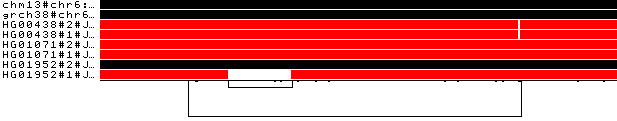
\includegraphics[width=\linewidth, trim=0 +1.9cm 0cm 0cm]{fig/extract_viz_draw_position_untangle/chr6_pan_fa_a2fb268_4030258_6a1ecc2_smooth_C4_sorted_z}
            \end{subfigure} \\
            \begin{subfigure}[t]{0.5\textwidth}
                \centering
                \caption{}
                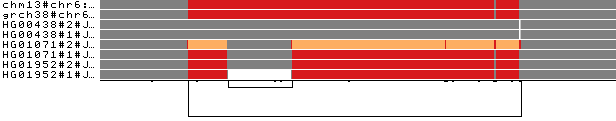
\includegraphics[width=\linewidth, trim=0 +1.9cm 0cm 0cm]{fig/extract_viz_draw_position_untangle/chr6_pan_fa_a2fb268_4030258_6a1ecc2_smooth_C4_sorted_m}
            \end{subfigure}
        \end{tabular}
        %&
        \begin{tabular}{c}% if you add [t], than sub images are pushed down
            %\smallskip
            \\\\
            \begin{subfigure}[t]{0.5\textwidth}
                \centering
                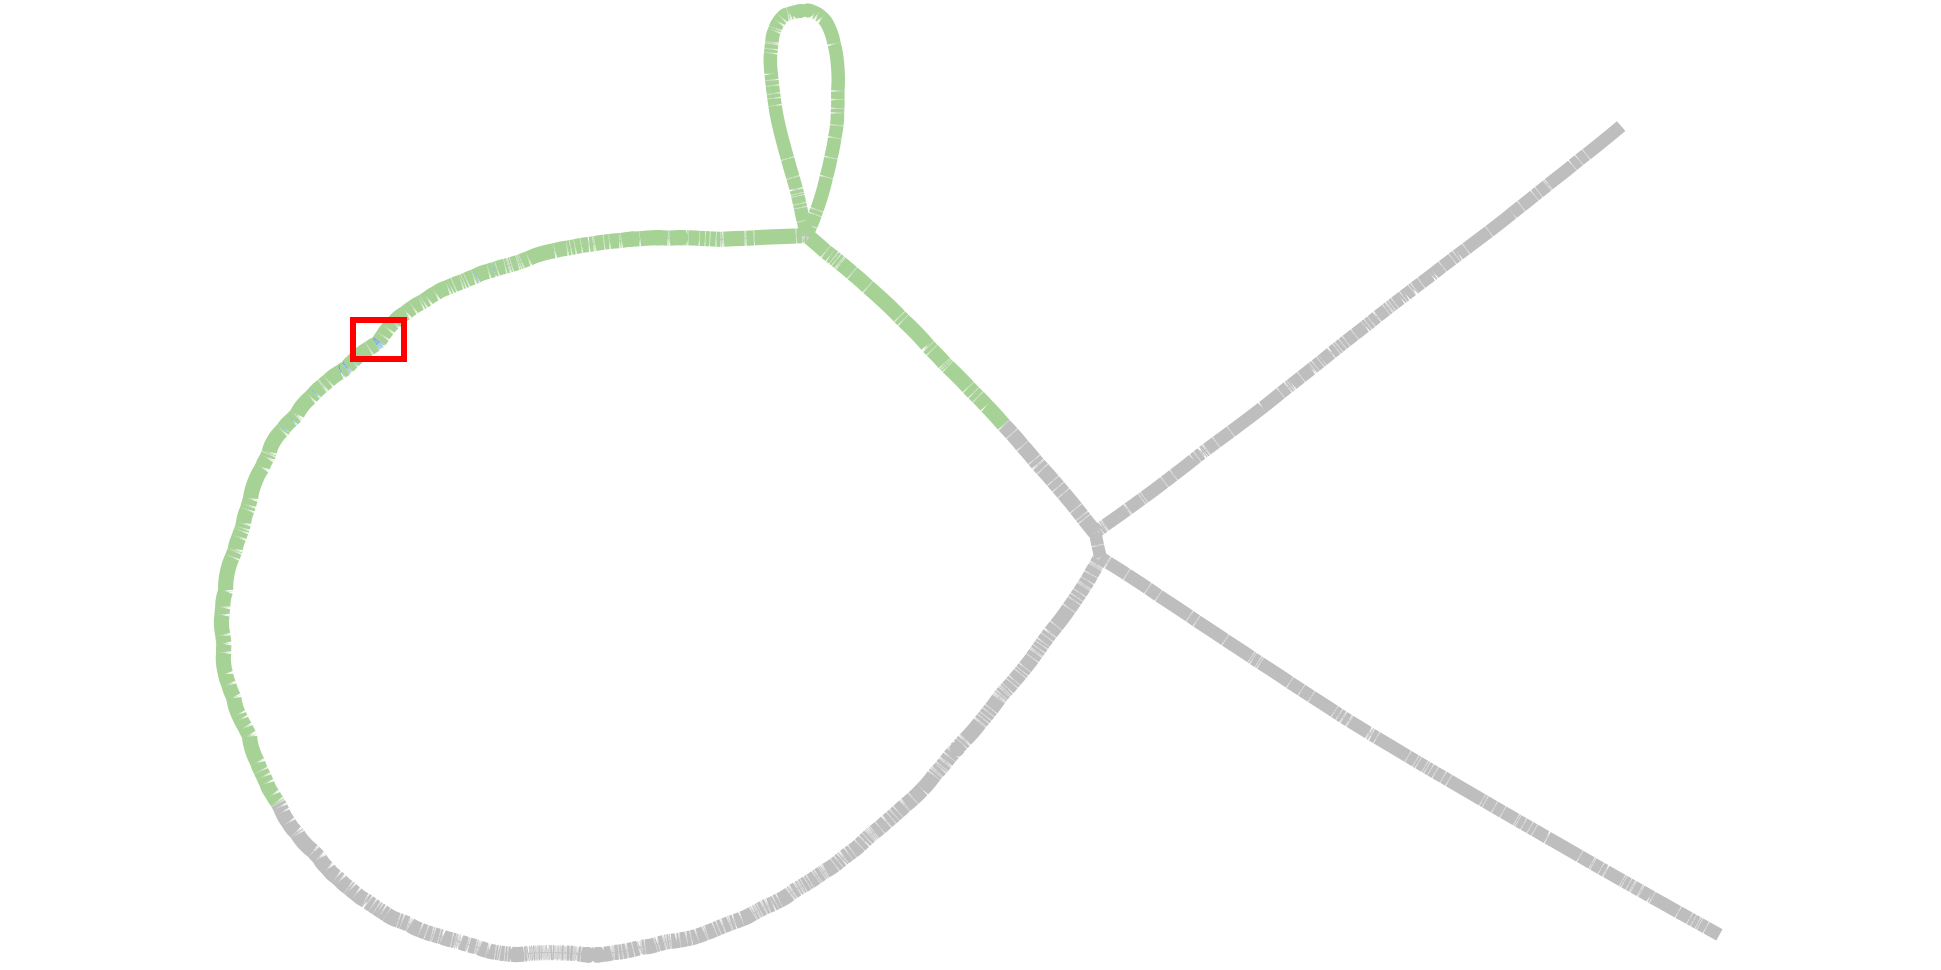
\includegraphics[width=0.65\linewidth, trim=0 +2cm 0 0.5cm]{fig/extract_viz_draw_position_untangle/chr6_pan_fa_a2fb268_4030258_d9f1245_smooth_gfa_C4_sorted_bandage}
                \caption{}
            \end{subfigure}
            \\\\
            \begin{subfigure}[t]{0.5\textwidth}
                \centering
                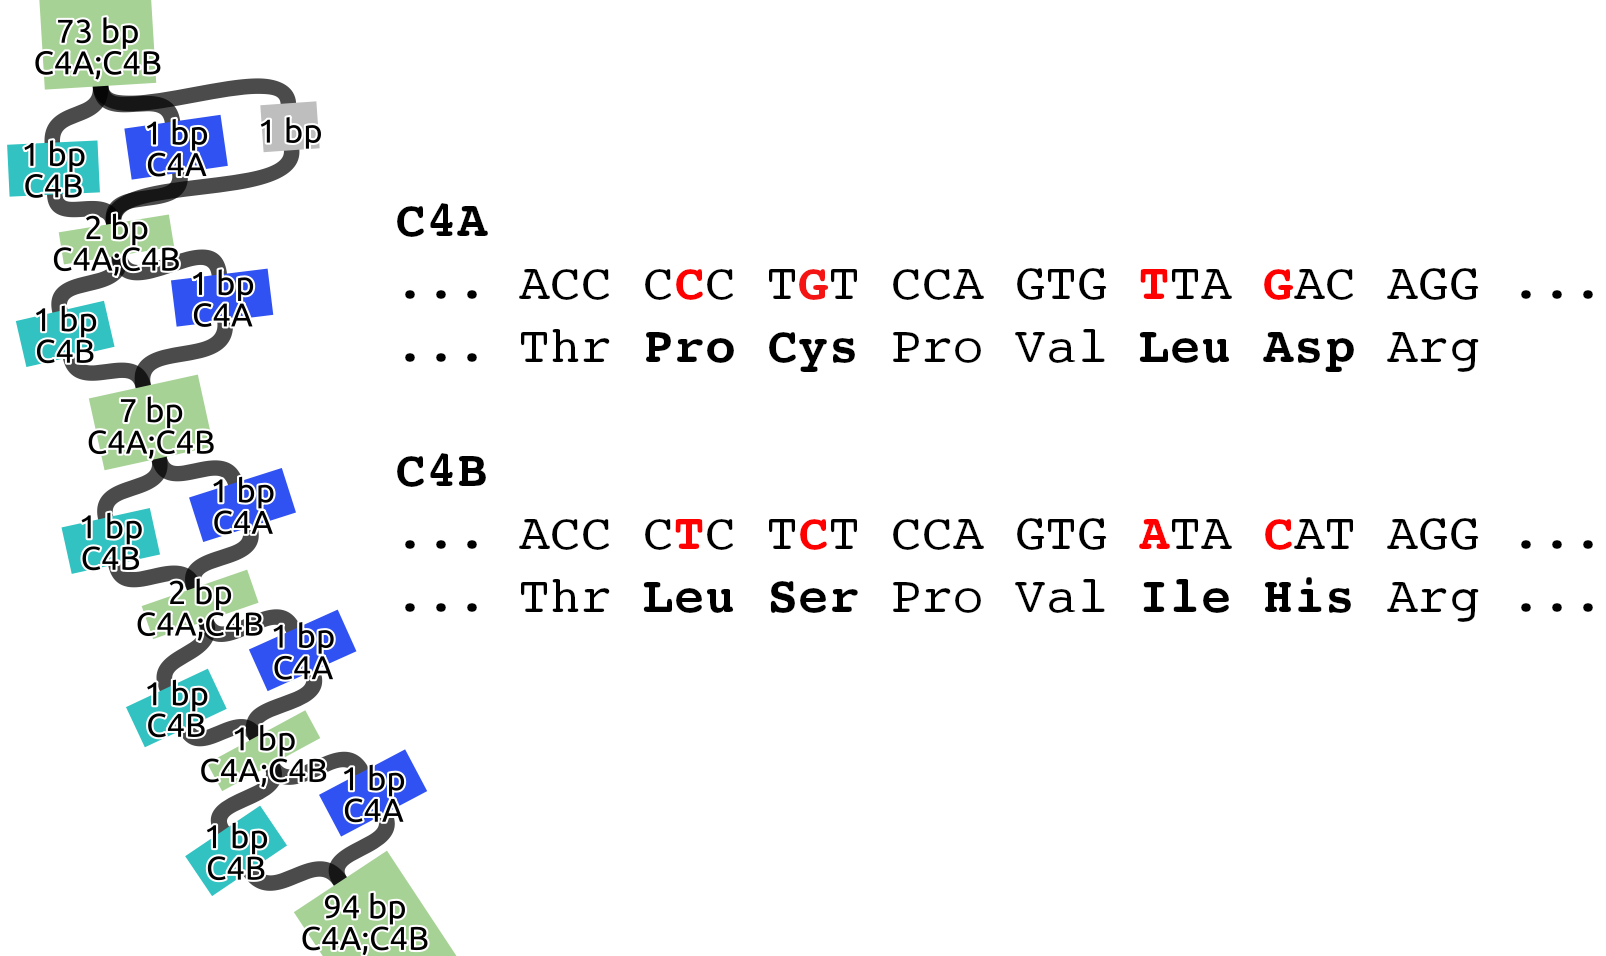
\includegraphics[width=0.65\linewidth, trim=0 +8cm 0 0.5cm]{fig/extract_viz_draw_position_untangle/chr6_pan_fa_a2fb268_4030258_d9f1245_smooth_gfa_C4_sorted_bandage_zoom_in}
                \caption{}
            \end{subfigure}
        \end{tabular}\\
        \begin{subfigure}[t]{1.0\textwidth}
            \centering
            \caption{}
            \begin{center}
                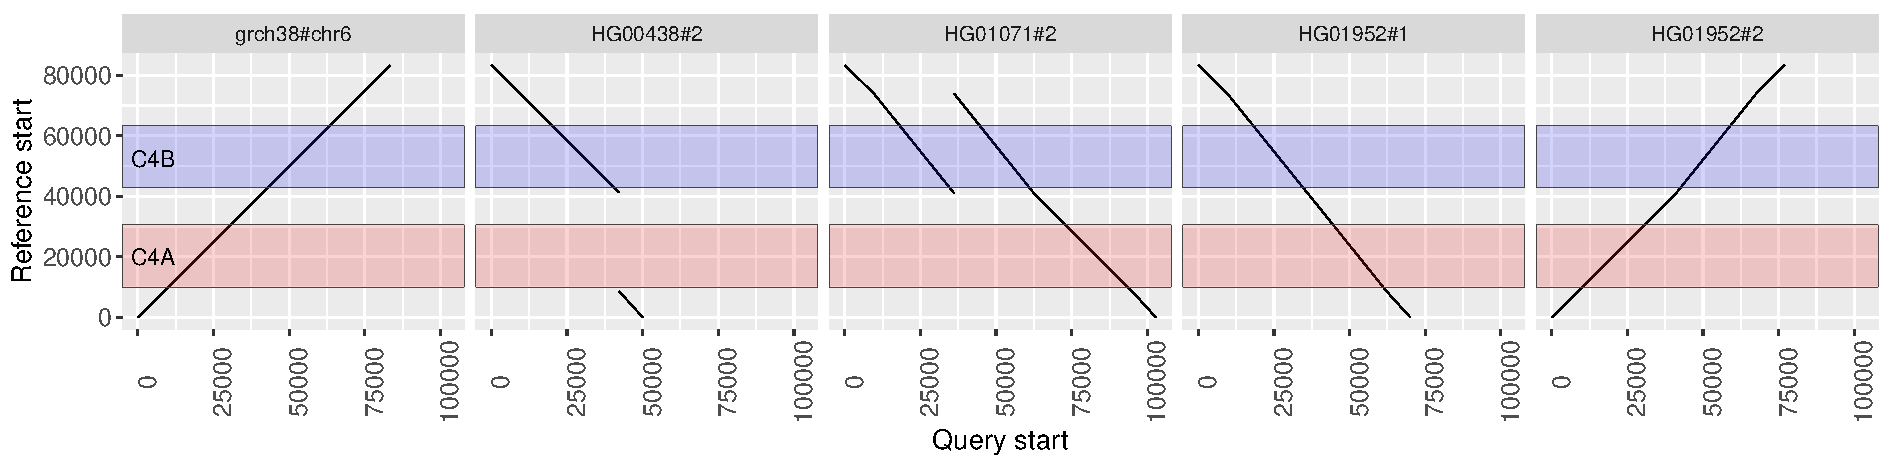
\includegraphics[width=\linewidth, trim=0cm 0.9cm -2.5cm 0.5cm]{fig/extract_viz_draw_position_untangle/chr6_pan_fa_a2fb268_4030258_6a1ecc2_smooth_C4_sorted_untangle_bed}
            \end{center}
        \end{subfigure} \\
        %\hline
    \end{tabular}
    \caption{
        Visualizing the \REVIEWED{major histocompatibility complex (MHC) and complement component 4 (C4)} pangenome graphs. \textbf{(a)} \textit{odgi draw} layout of the MHC pangenome graph extracted from a whole human pangenome graph of 90 haplotypes.
        \REVIEWED{The MHC locus is located on the human chromosome 6 and it encodes molecules involved in antigen presentation, inflammation regulation, the complement system, and the innate and adaptive immune responses~\citep{Shiina2009}.}
        The red rectangle highlights the C4 region\REVIEWED{, which encodes proteins involved in the complement system.}
        \textbf{(b-e)} \textit{odgi viz} visualizations of the C4 pangenome graph, where 8 paths are displayed: 2 reference genomes (chm13 and grch38 on the top) and 6 haplotypes of 3 individuals.
        \textbf{(b)} \textit{odgi viz} default modality: the image shows a quite linear graph.
        The longer links at the bottom indicate the presence of a structural variant (long link) with another structural variant nested inside it (short link on the left).
        Indeed, human C4 exists as 2 functionally distinct genes, \textit{C4A} and \textit{C4B}, which both vary in structure and copy number~\citep{Sekar_2016}. The longer link indicates that the copy number status varies across the haplotypes represented in the pangenome.
        Moreover, \textit{C4A} and \textit{C4B} genes segregate in both long and short genomic forms, distinguished by the presence or absence of a human endogenous retroviral (HERV) sequence, as also highlighted by the short nested link on the left.
        \textbf{(c)} Color by path position. %: the color gradients are smooth, highlighting that its node are well sorted in 1 dimension.
        The top two reference genomes and 2 haplotypes (HG01952\#2) go from left to right, while 5 haplotypes go in the opposite direction, as indicated by the black color on their left.
        \textbf{(d)} \textit{odgi viz} color by strandness: the red paths indicate the haplotypes that were assembled in reverse with respect to the 2 reference genomes.
        \textbf{(e)} \textit{odgi viz} color by node depth: using the Spectra color palette with 4 levels of node depths, white indicates no depth, while grey, red, and yellow indicate depth 1, 2, and greater than or equal to 3, respectively.
        Coloring by node depth, we can see that the two references present two different allele copies of the C4 genes, both of them including the HERV sequence.
        The entirely grey paths have one copy of these genes.
        HG01071\#2 presents 3 copies of the \textit{locus} (orange), of which one contains the HERV sequence (gray in the middle of the orange).
        In HG01952\#1, the HERV sequence is absent.
        \textbf{(f)} \REVIEWED{Layout of the C4 pangenome graph made with the \textit{Bandage} tool~\citep{Wick_2015} and} annotated by using \textit{odgi position}. Green nodes indicate the C4 genes. The red rectangle highlights the regions where \textit{C4A} and \textit{C4B} genes differ.
        \textbf{(g)} Annotated \textit{Bandage} layout of the C4 region where \textit{C4A} and \textit{C4B} genes differ due to single nucleotide variants leading to changes in the encoded protein sequences. Node labels were annoted by using \textit{odgi position}.
        \textbf{(h)} Visualization of \textit{odgi untangle} output in the C4 pangenome graph: the plots show the copy number status of the sequences in the C4 region with respect to the grch38 reference sequence, making clear, for example, that in HG00438\#2, the \textit{C4A} gene is missing. \vspace{-1em}
    }
    \label{fig:odgi_viz}
\end{figure*}


%\begin{figure*}[h!]
%    \begin{subfigure}[t]{.50\linewidth}
%        \caption{}
%        \centering
%        % include first image
%        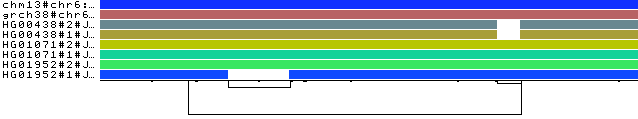
\includegraphics[width=\linewidth, trim=0 +1.5cm -0.5cm 0.5cm]{fig/extract_viz_draw_position_untangle/chr6_pan_fa_a2fb268_4030258_d9f1245_smooth_gfa_C4_sorted}
%        \label{fig:odgi_viz_default}
%    \end{subfigure}
%
%    \begin{subfigure}[t]{.50\linewidth}
%        \caption{}
%        \centering
%        % include second image
%        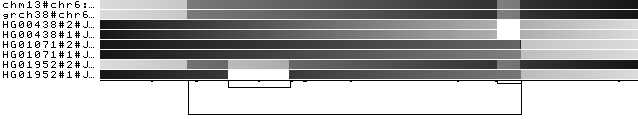
\includegraphics[width=\linewidth, trim=0 +1.5cm -0.5cm 0.5cm]{fig/extract_viz_draw_position_untangle/chr6_pan_fa_a2fb268_4030258_d9f1245_smooth_gfa_C4_sorted_du}
%        \label{fig:odgi_viz_color_by_path_pos}
%    \end{subfigure}
%
%    \begin{subfigure}[t]{.50\linewidth}
%        \caption{}
%        \centering
%        % include second image
%        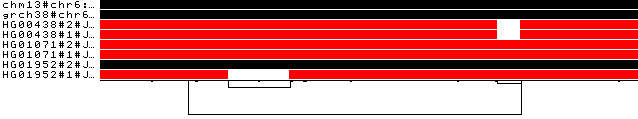
\includegraphics[width=\linewidth, trim=0 +1.5cm -0.5cm 0.5cm]{fig/extract_viz_draw_position_untangle/chr6_pan_fa_a2fb268_4030258_d9f1245_smooth_gfa_C4_sorted_z}
%        \label{fig:odgi_viz_color_by_inversion_rate}
%    \end{subfigure}
%
%    \begin{subfigure}[t]{.50\linewidth}
%        \caption{}
%        \centering
%        % include fourth image
%        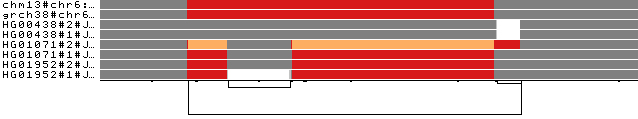
\includegraphics[width=\linewidth, trim=0 +1.5cm -0.5cm 0.5cm]{fig/extract_viz_draw_position_untangle/chr6_pan_fa_a2fb268_4030258_d9f1245_smooth_gfa_C4_sorted_m}
%        \label{fig:odgi_viz_color_by_path_depth}
%    \end{subfigure}
%    \begin{subfigure}[t]{.50\linewidth}
%        \caption{}
%        \centering
%        % include first image
%        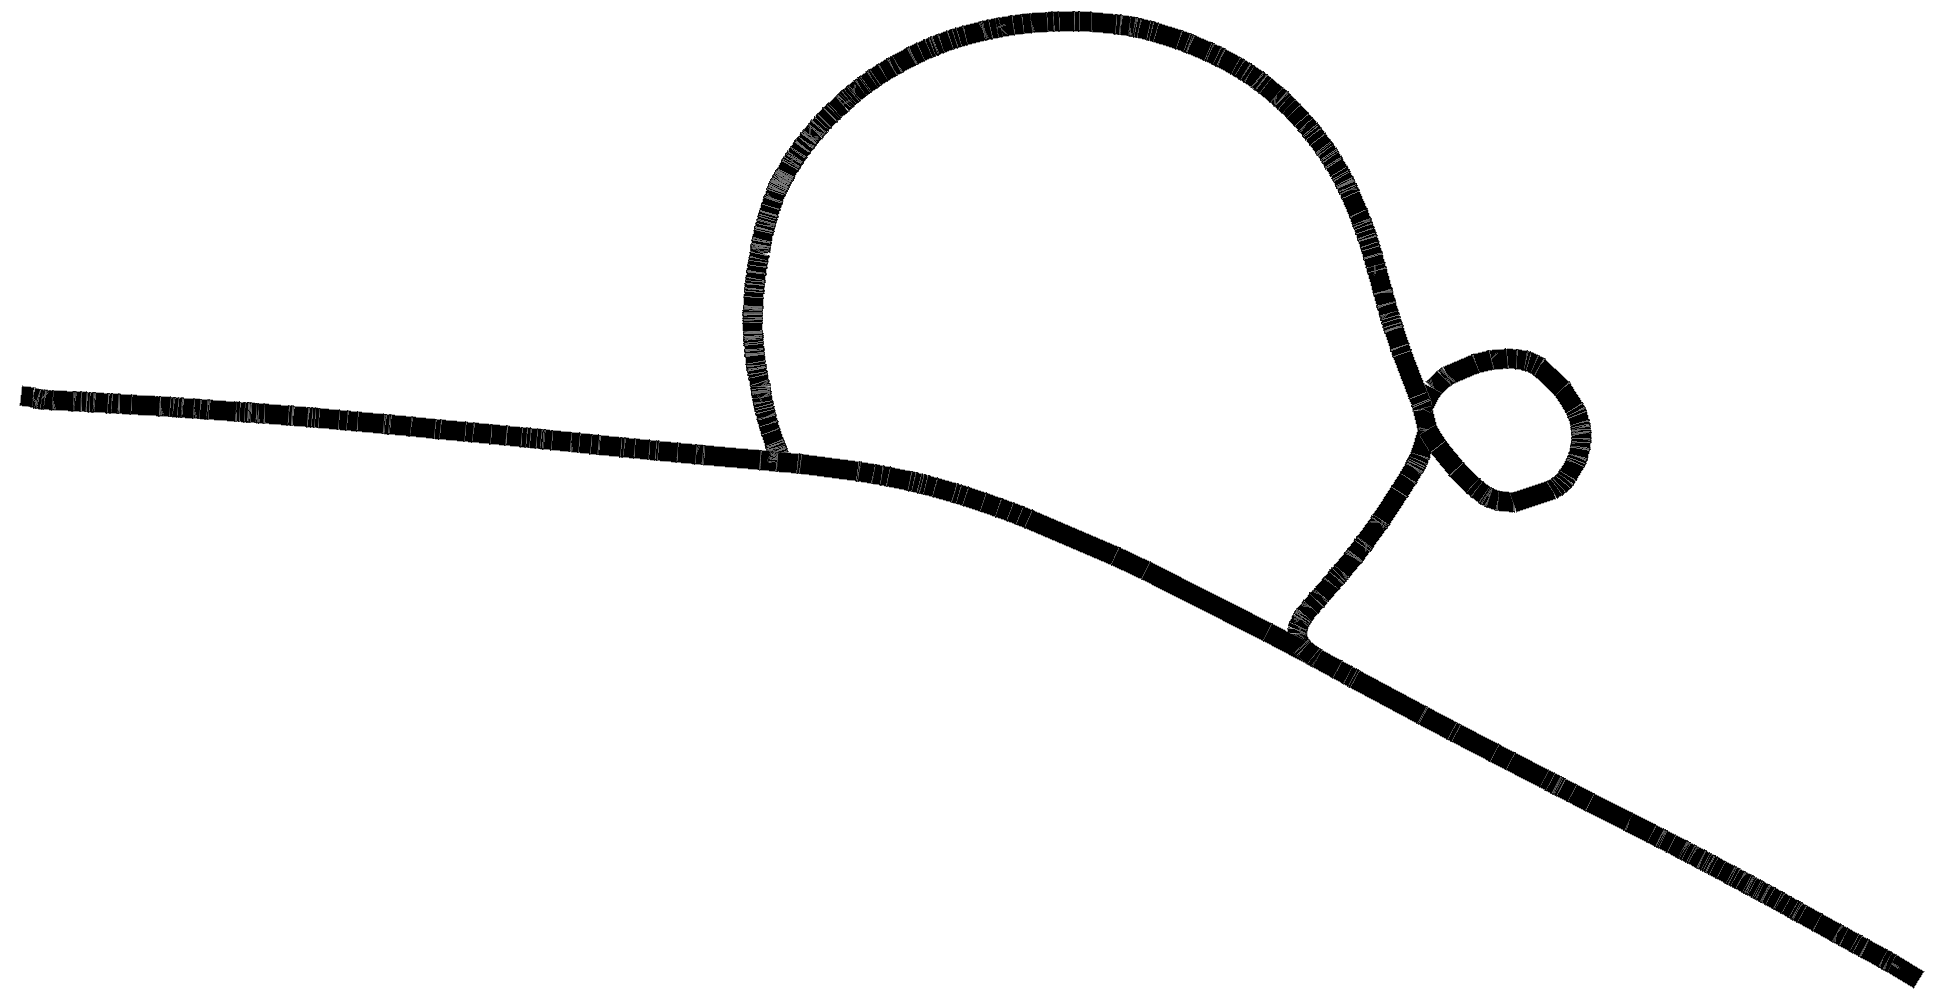
\includegraphics[width=0.5\linewidth, trim=0 +2cm 0 0.5cm]{fig/extract_viz_draw_position_untangle/chr6_pan_fa_a2fb268_4030258_d9f1245_smooth_gfa_C4_sorted_layout}
%        \label{fig:odgi_viz_default2}
%    \end{subfigure}
%    \begin{subfigure}[t]{.50\linewidth}
%        \caption{}
%        \centering
%        % include second image
%        %todo BANDAGE
%        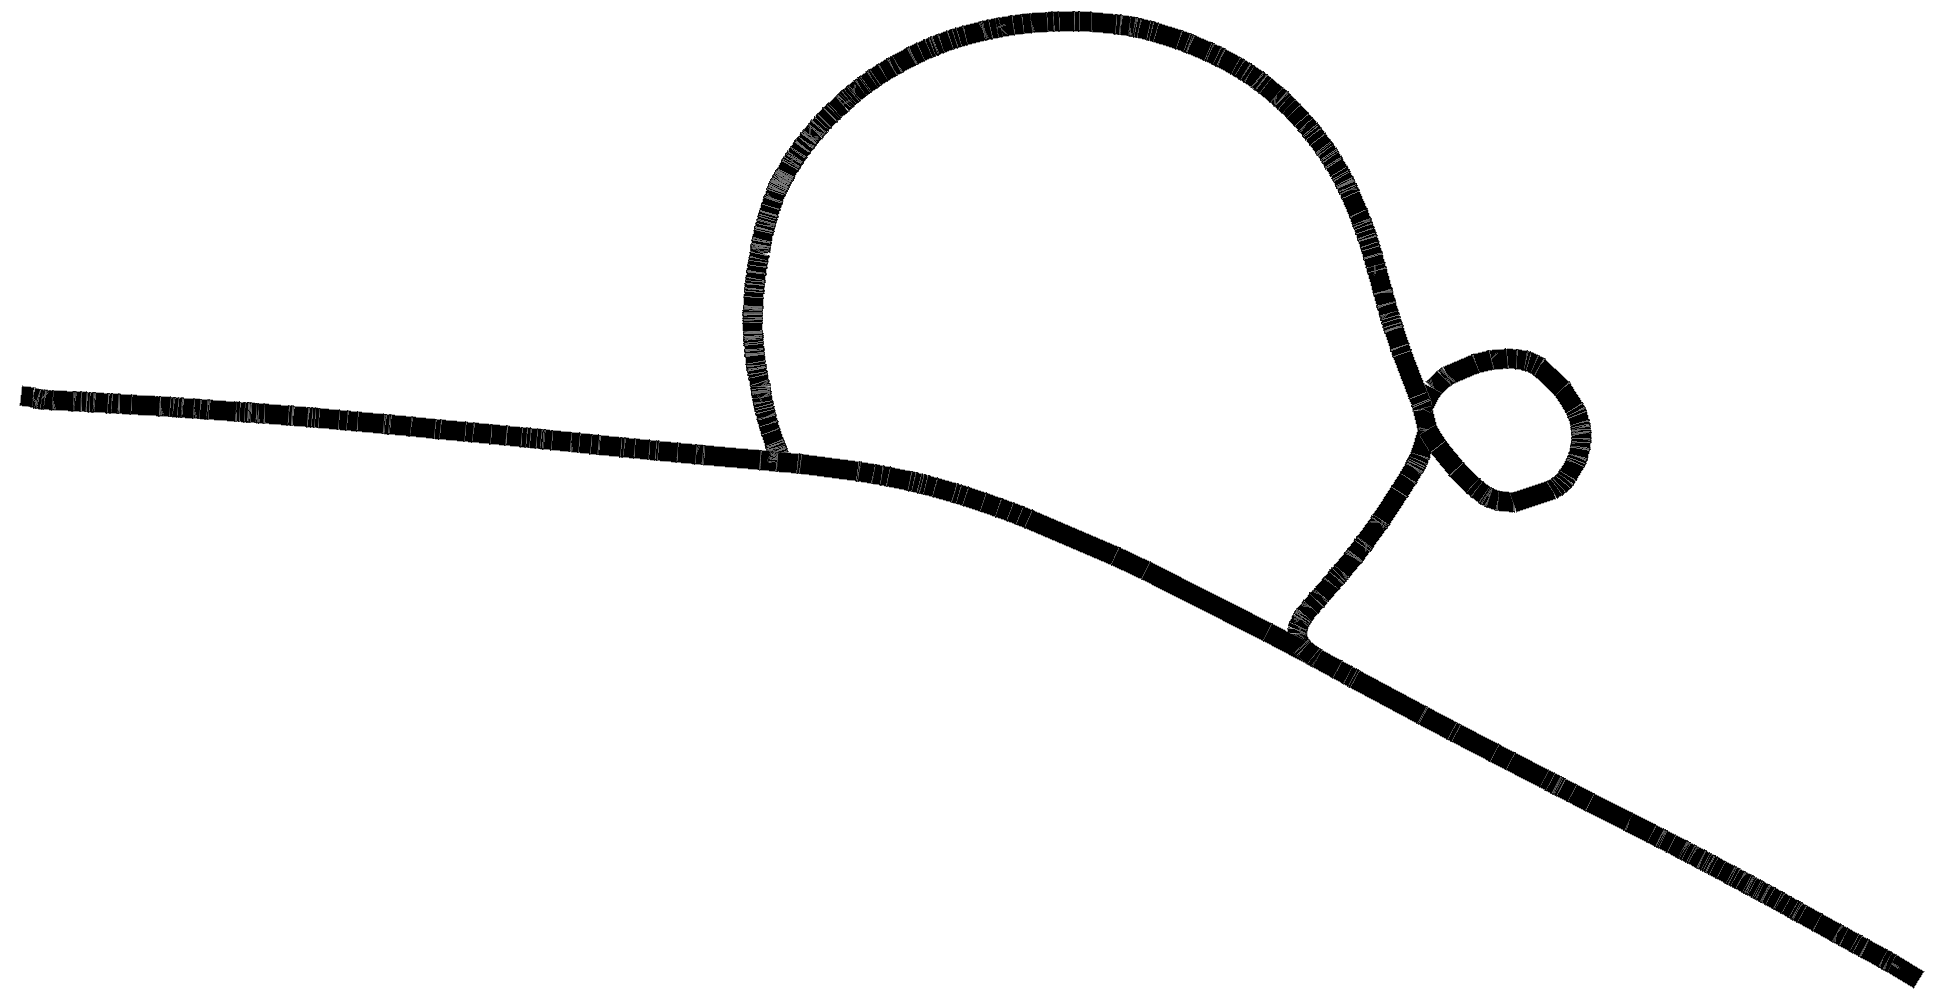
\includegraphics[width=0.5\linewidth, trim=0 +1.5cm -0.5cm 0.5cm]{fig/extract_viz_draw_position_untangle/chr6_pan_fa_a2fb268_4030258_d9f1245_smooth_gfa_C4_sorted_layout}
%        \label{fig:odgi_viz_color_by_inversion_rate2}
%    \end{subfigure}
%
%    \caption{
%        Visualizing the complement component 4 (C4) pangenome graph extracted from a whole human pangenome graph of 90 haplotypes.
%        In all visualizations, 8 paths are displayed: 2 reference genomes (chm13 and grch38 on the top) and 6 haplotypes of 3 individuals.
%        \textbf{(a)} default modality: the image shows a quite linear graph.
%        The longer links at the bottom indicate the presence of a structural variant (long link) with another structural variant nested inside it (short link on the left).
%        Indeed, human C4 exists as 2 functionally distinct genes, C4A and C4B, which both vary in structure and copy number \citep{Sekar_2016}. The longer link indicates that the copy number status varies across the haplotypes represented in the pangenome.
%        Moreover, C4A and C4B genes segregate in both long and short genomic forms, distinguished by the presence or absence of a human endogenous retroviral (HERV) sequence, as also highlighted by the short nested link on the left.
%        \textbf{(b)} color by path position: the color gradients are smooths, highlighting that its node are well sorted in 1 dimension.
%        The top two reference genomes and 2 haplotypes (with name starting with HG01952\#2) go from left to right, while 5 haplotypes go in the opposite direction, as indicated by the black color on their left.
%        \textbf{(c)} color by strandness: the red paths indicate the haplotypes that were assembled in reverse with respect to the 2 reference genomes.
%        \textbf{(d)} color by path depth: using the Spectra color palette with 4 level of path depths, white indicates no depth, while grey, red, and yellow indicate depth 1, 2, and greater than or equal to 3, respectively.
%        Coloring by path depth, we can see that the two references present two different allele copies of the C4 genes, both of them including the HERV sequence.
%        The entirely grey paths have one copy of these genes.
%        The path with name starting with HG01071\#2 presents 3 copies of the genes (indicated by the orange color), of which only 1 with the HERV sequence (gray color in the middle of the orange region).
%        In the haplotype with the name starting with HG01952\#1, the HERV sequence is absent.
%    }
%    \label{fig:odgi_viz}
%\end{figure*}

%\begin{figure}[ht!]
	\begin{subfigure}{\linewidth}
		\caption{}
		\centering
		% include second image
		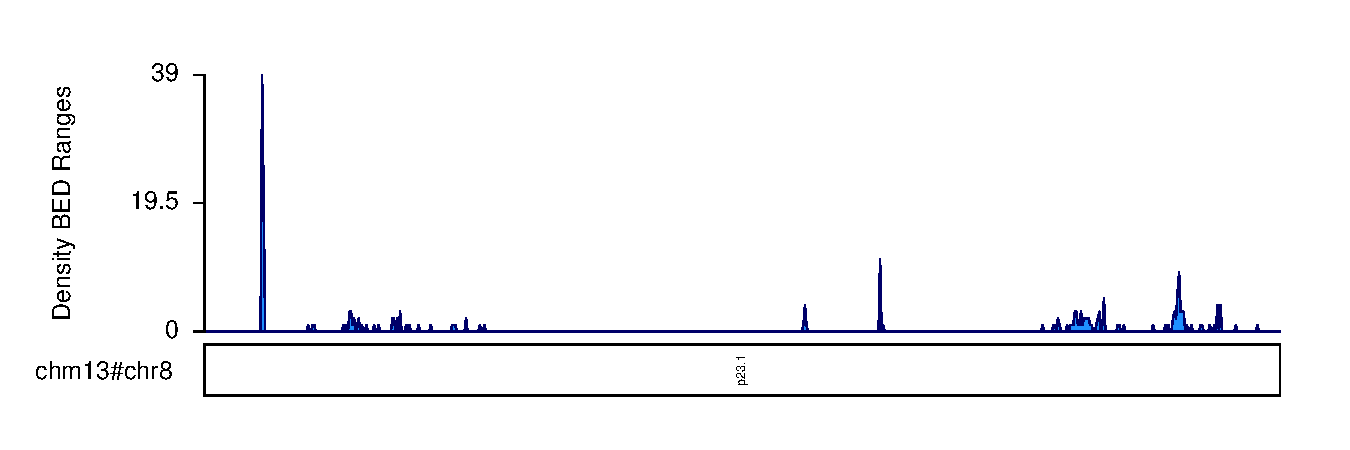
\includegraphics[width=1.0\linewidth, trim=0cm 2.75cm 0cm 0cm]{fig/tips/chr8_chm13_beta_defensin_locus_odgi_tips_w50000_karyoploteR}
		\label{fig:tips-karyo}
	\end{subfigure}
	%	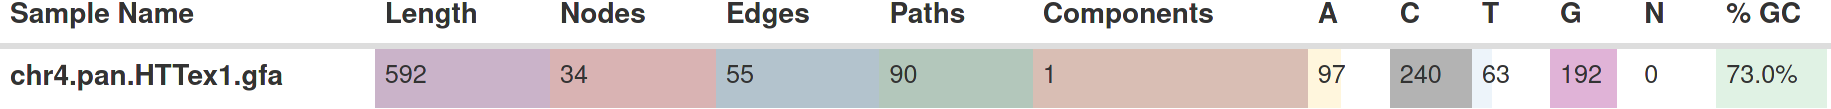
\includegraphics[width=\linewidth]{fig/metrics/chr4.pan.HTTex1.gfa.multiqc_odgi_stats.png}
	\caption{Visualizing the contigs of a beta-defensin locus pangenome graph. (\textbf{a}) Breakpoint ranges of the contigs in the beta-defensin locus pangenome graph of 90 haplotypes relative to CHM13. The \textit{odgi tips} results are visualized as the density of BED ranges across the whole \textit{p23.1} cytoband. The high peak at the beginning of \textit{p23.1} indicates that 39 contigs of the graph broke there relative to CHM13. (\textbf{b}) \FIXME{ADD VIZ AS SOON AS THE SORTING IS FINISHED.}}
	\label{fig:tips}
\end{figure}


%\begin{figure}[h!]
	\begin{subfigure}{\linewidth}
		%\caption{}
		\centering
		% include first image
		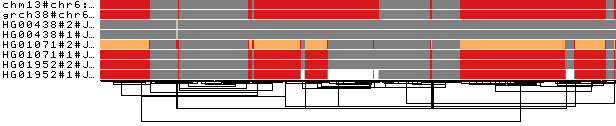
\includegraphics[width=1.0\linewidth, trim=-0cm 2cm 0 0cm]{fig/sorting/chr6_pan_fa_a2fb268_4030258_6a1ecc2_smooth_C4_bad_sorted}
		\label{fig:bad-sorting}
	\end{subfigure}
%	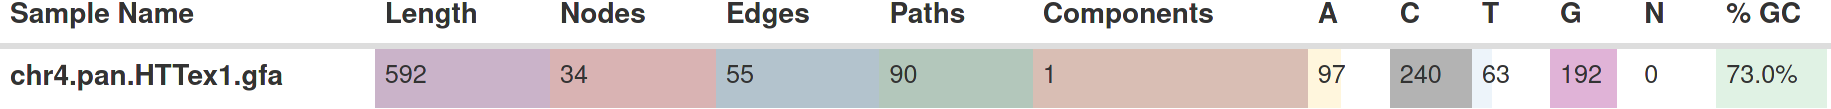
\includegraphics[width=\linewidth]{fig/metrics/chr4.pan.HTTex1.gfa.multiqc_odgi_stats.png}
	\caption{
		Visualization of a poorly sorted C4 pangenome graph.
		Same \textit{odgi viz} visualization as the one shown in Fig.~\ref{fig:odgi_viz}\textbf{e}, but with a graph where the bad node order hides the underlying copy number variation status present in the C4 region.
	}
	\label{fig:sorting}
\end{figure}




% Figure: small graph with all the stats shown. A screenshot of MultiQC, visualize summary per bin somehow, R visualizations of degree and depth HTT exon 1 as tiny example graph

\section{Discussion}
Pangenome graphs stand to become a ubiquitous model in genomics thanks to their capability to represent any genetic variant without being affected by reference bias~\citep{Eizenga_2020}.
However, despite this great potential, their spread is impeded by the lack of tools capable of managing and analyzing pangenome graphs easily and efficiently.

ODGI is a state-of-the-art tool suite that enables users to explore and discover the underlying biology in pangenomes graphs, filling the gap that made pangenomic analyses difficult.
It provides tools to easily transform, analyze, simplify, validate, and visualize pangenome graphs at large scale.
In particular, lifting over annotations and linearizing nested graph structures place the suite as the bridge between traditional linear reference genome analysis and pangenome graphs.
With the increased adoption of long read sequencing we expect pangenomic tools to become increasingly common in \REVIEWED{the genomic studies at different taxonomic levels and} in biomedical research.
Particularly for targets that involve complex variation, such as cancer\REVIEWED{~\citep{CompPan2016}}, plant genomics\REVIEWED{~\citep{Bayer2020}} and metagenomics\REVIEWED{~\citep{Zhong2021}}, ODGI will facilitate disentangling,
describing and analyzing a much larger set of variation than previously was possible with tools that depend on short reads and reference genomes.
Furthermore, users can even consider ODGI as a framework, taking advantage of its algorithms to develop new and more advanced tools that work on pangenome graphs,
thus expanding the type of possible pangenomic analyses available to the scientific community.

\REVIEWED{[1,10]While ODGI does not construct graphs from scratch nor is is capable of extending them, ODGI[1,10]} is already the backbone of the Pangenome Graph Builder pipeline~\citep{pggb}.
Its static, large-scale 1D and 2D visualizations of the pangenome graphs allow an unprecedented high-level perspective on variation in pangenomes, and have also been critical in the development of pangenome graph building methods.  %the underlying structure and any problems in graph construction.
However, an interactive solution that combines the 1D and 2D layout of a graph with annotation and read mapping information across different zoom levels is still missing.
Recent interactive browsers are reference-centric~\citep{Beyer2019, Yokoyama2019, Durant2021, Liang2021} or focus primarily on 2D~\citep{Wick_2015, Gonnella2018}.
Our graph sorting and layout algorithms can provide the foundation for future tools of this type.
We plan to focus on using these learned models to detect structural variation and assembly errors.
%In ODGI, we provide a graph layout algorithm that can become a backbone of such tools, as is already the case for \textit{gfaestus}~\citep{gfaestus} %\footnote{\url{https://github.com/chfi/gfaestus}},
%which currently relies on the \textit{odgi layout} output for its interactive 2D graph visualization.

ODGI has allowed us to explore \textit{context mapping} deconvolution of pangenome graph structures via the path jaccard metric.
This resolves a major conceptual issue that has strongly guided existing algorithms to construct pangenome graphs.
Previously, great efforts have been made to prevent the ``collapse'' of non-orthologous sequences in the graph topology itself  \citep{Li:2020}.
This has been seen as essential to making these new bioinformatic models interpretable.
While our presentation is primarily qualitative, our work demonstrates that we can mitigate this issue by exploiting the pangenome graph not as a static reference, but as a dynamic model of the mutual alignment of many \REVIEWED{[1.2] genomic sequences [1.2]}.
Because pangenome graphs can contain complete genomes, we are able to query them to polarize the information they contain in easily-interpretable and reusable pairwise formats that are widely supported in bioinformatics.
ODGI also projects variation graphs into vector and matrix representations that allow the direct application of machine learning and statistical models to the pangenome.
%By providing convenient linearizations and matrix transformations, ODGI also provides an interface for machine learning on pangenomes.
%can be linearized into feature vector or matrix form, and ODGI thus provides a natural interface for machine learning and statistical methods that operate directly on data of this shape.
We expect that ODGI will provide a reference interface between pangenomic and genomic approaches to understanding genome variation.

%To understand this model, we query it using any reference that it contains.

%Our future work will focus on further extensions of this topic.

%Here, we present only qualitative evaluation of this result, but our future work will focus on exploiting this mechanism to simplify and aid the interpretation of large pangenomes.

%ODGI aims to be a reference implementation for many pangenome related operations, thus future work will be focused on multiple directions.
%First, we will expand its metadata capabilities to annotate large pangenome graphs.
%Futhermore, we will improve RDF support for annotation in the in-memory graph~\citep{Yokoyama2020} and allow for federated queries on pangenome graphs.
%Finally, we will explore the addition of support for RNA sequences and proteins to extend the application of pangenomic approaches to other levels in the genetic information flow from DNA to phenotype.





%So far, ODGI has not been applied to graphs build from scWGS~\citep{Zhuo2021} data. Each cell would be represented as a path in the graph, the path depth would be very high.
%As ODGI was designed to deal with the path depth of human pangenome graphs, it remains to be seen, if it will work equally well with scWGS data.

\section*{Acknowledgements}

We thank members of the HPRC Pangenome Working Group for their insightful discussion and feedback, and members of the HPRC production teams for their development of resources used in our exposition.

\section*{Funding}

We gratefully acknowledge support from NIH/NIDA U01DA047638 (EG) and NIH/NIGMS R01GM123489 (EG and PP).
SH acknowledges funding from the Central Innovation Programme (ZIM) for SMEs of the Federal Ministry for Economic Affairs and Energy of Germany. SN acknowleges Germany’s Excellence Strategy (CMFI), EXC-2124 and (iFIT) - EXC 2180 – 390900677.
This work was supported by the BMBF-funded de.NBI Cloud within the German Network for Bioinformatics Infrastructure (de.NBI) (031A537B, 031A533A, 031A538A, 031A533B, 031A535A, 031A537C, 031A534A, 031A532B).
\linebreak
\linebreak
\REVIEWED{\textit{Conflict of Interest}: the authors declare no competing interests.}


\section*{Data availability}

%Data used to build human pangenome graphs: \url{https://github.com/human-pangenomics/HPP_Year1_Data_Freeze_v1.0}. 
%The graphs we generated the figures from: \url{https://s3-us-west-2.amazonaws.com/human-pangenomics/index.html?prefix=pangenomes/scratch/2021_11_04_pggb_wgg.87/}.
Code and links to data resources used to build this manuscript and its figures, can be found in the paper's public repository: \url{https://github.com/pangenome/odgi-paper}.


\bibliographystyle{natbib}
%\bibliographystyle{achemnat}
%\bibliographystyle{plainnat}
%\bibliographystyle{abbrv}
%\bibliographystyle{bioinformatics}
%
%\bibliographystyle{plain}
%
\bibliography{document}


% \begin{thebibliography}{}

% \bibitem[Bofelli {\it et~al}., 2000]{Boffelli03}
% Bofelli,F., Name2, Name3 (2003) Article title, {\it Journal Name}, {\bf 199}, 133-154.

% \bibitem[Bag {\it et~al}., 2001]{Bag01}
% Bag,M., Name2, Name3 (2001) Article title, {\it Journal Name}, {\bf 99}, 33-54.

% \bibitem[Yoo \textit{et~al}., 2003]{Yoo03}
% Yoo,M.S. \textit{et~al}. (2003) Oxidative stress regulated genes
% in nigral dopaminergic neurnol cell: correlation with the known
% pathology in Parkinson's disease. \textit{Brain Res. Mol. Brain
% Res.}, \textbf{110}(Suppl. 1), 76--84.

% \bibitem[Lehmann, 1986]{Leh86}
% Lehmann,E.L. (1986) Chapter title. \textit{Book Title}. Vol.~1, 2nd edn. Springer-Verlag, New York.

% \bibitem[Crenshaw and Jones, 2003]{Cre03}
% Crenshaw, B.,III, and Jones, W.B.,Jr (2003) The future of clinical
% cancer management: one tumor, one chip. \textit{Bioinformatics},
% doi:10.1093/bioinformatics/btn000.

% \bibitem[Auhtor \textit{et~al}. (2000)]{Aut00}
% Auhtor,A.B. \textit{et~al}. (2000) Chapter title. In Smith, A.C.
% (ed.), \textit{Book Title}, 2nd edn. Publisher, Location, Vol. 1, pp.
% ???--???.

% \bibitem[Bardet, 1920]{Bar20}
% Bardet, G. (1920) Sur un syndrome d'obesite infantile avec
% polydactylie et retinite pigmentaire (contribution a l'etude des
% formes cliniques de l'obesite hypophysaire). PhD Thesis, name of
% institution, Paris, France.

% \end{thebibliography}
\end{document}
